%% abtex2-modelo-trabalho-academico.tex, v-1.9.2 laurocesar
%% Copyright 2012-2014 by abnTeX2 group at http://abntex2.googlecode.com/ 
%%
%% This work may be distributed and/or modified under the
%% conditions of the LaTeX Project Public License, either version 1.3
%% of this license or (at your option) any later version.
%% The latest version of this license is in
%%   http://www.latex-project.org/lppl.txt
%% and version 1.3 or later is part of all distributions of LaTeX
%% version 2005/12/01 or later.
%%
%% This work has the LPPL maintenance status `maintained'.
%% 
%% The Current Maintainer of this work is the abnTeX2 team, led
%% by Lauro César Araujo. Further information are available on 
%% http://abntex2.googlecode.com/
%%
%% This work consists of the files abntex2-modelo-trabalho-academico.tex,
%% delo-include-comandos and abntex2-modelo-references.bib
%%

% ------------------------------------------------------------------------
% ------------------------------------------------------------------------
% abnTeX2: Modelo de trabalho Academico (tese de doutorado, dissertacao de
% mestrado e trabalhos monograficos em geral) em conformidade com 
% ABNT NBR 14724:2011: Informacao e documentacao - Trabalhos academicos -
% Apresentacao
% ------------------------------------------------------------------------
% ------------------------------------------------------------------------

\documentclass[
	% -- opções da classe memoir --
	12pt,				% tamanho da fonte
%	openright,			% capítulos começam em pág ímpar (insere página vazia caso preciso)
%	twoside,			% para impressão em verso e anverso. Oposto a oneside
	oneside,
	a4paper,			% tamanho do papel. 
	% -- opções da classe abntex2 --
	%chapter=TITLE,		% títulos de capítulos convertidos em letras maiúsculas
	%section=TITLE,		% títulos de seções convertidos em letras maiúsculas
	%subsection=TITLE,	% títulos de subseções convertidos em letras maiúsculas
	%subsubsection=TITLE,% títulos de subsubseções convertidos em letras maiúsculas
	% -- opções do pacote babel --
	english,			% idioma adicional para hifenização
	brazil				% o último idioma é o principal do documento
	]{abntex2ufop} % classe abntex2ufop para escrita de trabalhos academicos

% ---
% Pacotes básicos 
% ---
\usepackage{lmodern}			% Usa a fonte Latin Modern			
\usepackage[T1]{fontenc}		% Selecao de codigos de fonte.
\usepackage[utf8]{inputenc}		% Codificacao do documento (conversão automática dos acentos)
\usepackage{lastpage}			% Usado pela Ficha catalográfica
\usepackage{indentfirst}		% Indenta o primeiro parágrafo de cada seção.
\usepackage{color}				% Controle das cores
\usepackage[table,xcdraw]{xcolor}
\usepackage{graphicx}			% Inclusão de gráficos
\usepackage{microtype} 			% para melhorias de justificação
\usepackage{supertabular}       % tabela na capa do dosudo apt-get install texlive texlive-latex3cumento
\usepackage{listings}
\usepackage{pdfpages}
\usepackage{csquotes}


\usepackage{float}
\floatstyle{plaintop}
\restylefloat{table}
% ---
		
% ---
% Pacotes adicionais, usados apenas no âmbito do Modelo Canônico do abnteX2 - pode ser removido

% ---
% Pacotes adicionais, usados no anexo do modelo de folha de identificação
% ---
\usepackage{multicol}
\usepackage{multirow}
\usepackage{lipsum}				% para geração de dummy text
% ---

% ---
% Pacotes de citações
% ---
\usepackage[brazilian,hyperpageref]{backref}	 % Paginas com as citações na bibliografia
\usepackage[alf]{abntex2cite}	% Citações padrão ABNT 6023

% ---
% CONFIGURACOES LISTAGEM DE CODIGOS
% ---

\definecolor{lightgray}{rgb}{.97,.97,.97}
\definecolor{darkgray}{rgb}{.4,.4,.4}
\definecolor{purple}{rgb}{0.65, 0.12, 0.82}

\lstdefinelanguage{Javascript}{
	keywords={typeof, new, true, false, catch, function, return, null, catch, switch, var, if, in, while, do, else, case, break, async},
	keywordstyle=\color{blue}\bfseries,
	ndkeywords={class, export, boolean, throw, implements, import, this, const},
	ndkeywordstyle=\color{darkgray}\bfseries,
	identifierstyle=\color{black},
	sensitive=false,
	comment=[l]{//},
	morecomment=[s]{/*}{*/},
	commentstyle=\color{purple}\ttfamily,
	stringstyle=\color{red}\ttfamily,
	morestring=[b]',
	morestring=[b]"
}

\lstset{
	language=Javascript,
	backgroundcolor=\color{lightgray},
	extendedchars=true,
	basicstyle=\footnotesize\ttfamily,
	showstringspaces=false,
	showspaces=false,
	numbers=left,
	numberstyle=\footnotesize,
	numbersep=9pt,
	tabsize=2,
	breaklines=true,
	showtabs=false,
	captionpos=b
}

% --- 
% CONFIGURAÇÕES DE PACOTES
% --- 

% ---
% Configurações do pacote backref
% Usado sem a opção hyperpageref de backref
\renewcommand{\backrefpagesname}{Citado na(s) página(s):~}
% Texto padrão antes do número das páginas
\renewcommand{\backref}{}
% Define os textos da citação
\renewcommand*{\backrefalt}[4]{
	\ifcase #1 %
		Nenhuma citação no texto.%
	\or
		Citado na página #2.%
	\else
		Citado #1 vezes nas páginas #2.%
	\fi}%
% ---

% ---
% Informações de dados para CAPA e FOLHA DE ROSTO
% ---
\titulo{RECONHECIMENTO AUTOMÁTICO DE ETIQUETAS IDENTIFICADORAS EM TARUGOS}
\autor{Antônio Henrique Alves Cardoso}
\local{Ouro Preto}
\data{junho de 2020}
\orientador{Filipe Augusto Santos Rocha, M.Sc.}
\coorientador{Thomás Vargas Barsante e Pinto}
\instituicao{Universidade Federal de Ouro Preto - UFOP}
\escolademinas{Escola de Minas}
\colegiado{Colegiado do curso de Engenharia de Controle e Automa{\c c}{\~a}o - CECAU}
\tipotrabalho{Monografia de Gradua{\c c}{\~a}o em Engenharia de Controle e Automa{\c c}{\~a}o }
% O preambulo deve conter o tipo do trabalho, o objetivo, 
% o nome da instituição e a área de concentração 
\preambulo{Monografia apresentada ao Curso de Engenharia de Controle e Automa{\c c}{\~a}o da Universidade Federal de Ouro Preto como parte dos requisitos para a obten{\c c}{\~a}o do Grau de Engenheiro de Controle e Automa{\c c}{\~a}o.}
% ---


% ---
% Configurações de aparência do PDF final

% alterando o aspecto da cor azul
\definecolor{blue}{RGB}{41,5,195}
% informações do PDF
\makeatletter
\hypersetup{
     	%pagebackref=true,
		pdftitle={\@title}, 
		pdfauthor={\@author},
    	pdfsubject={\imprimirpreambulo},
	    pdfcreator={LaTeX with abnTeX2},
		pdfkeywords={abnt}{latex}{abntex}{abntex2}{trabalho acadêmico}, 
		colorlinks=true,       		% false: boxed links; true: colored links
    	linkcolor=black,          	% color of internal links
    	citecolor=black,        		% color of links to bibliography
    	filecolor=magenta,      		% color of file links
		urlcolor=black,
		bookmarksdepth=4
}
\makeatother
% --- 

% --- 
% Espaçamentos entre linhas e parágrafos 
% --- 

% O tamanho do parágrafo é dado por:
\setlength{\parindent}{1.25cm}

% Controle do espaçamento entre um parágrafo e outro:
\setlength{\parskip}{0.2cm}  % tente também \onelineskip

% ---
% compila o indice
% ---
\makeindex
% ---

% ----
% Início do documento
% ----
\begin{document}

% Retira espaço extra obsoleto entre as frases.
\frenchspacing 

% ----------------------------------------------------------
% ELEMENTOS PRÉ-TEXTUAIS
% ----------------------------------------------------------
% \pretextual

% ---
% Capa
% ---
\imprimircapa
% ---

% ---
% Folha de rosto
% (o * indica que haverá a ficha bibliográfica)
% ---
\imprimirfolhaderosto*
% ---


% ---
% Inserir a ficha bibliografica
% ---

% Isto é um exemplo de Ficha Catalográfica, ou ``Dados internacionais de
% catalogação-na-publicação''. 
% Porém, a biblioteca da sua universidade lhe fornecerá um PDF
% com a ficha catalográfica definitiva após a defesa do trabalho. Quando estiver
% com o documento, salve-o como PDF no diretório do seu projeto e substitua todo
% o conteúdo de implementação deste arquivo pelo comando abaixo que está comentado 
% (nao se esqueça de comentar o antigo ambiente de ficha catalográfica):
%
\begin{fichacatalografica}
    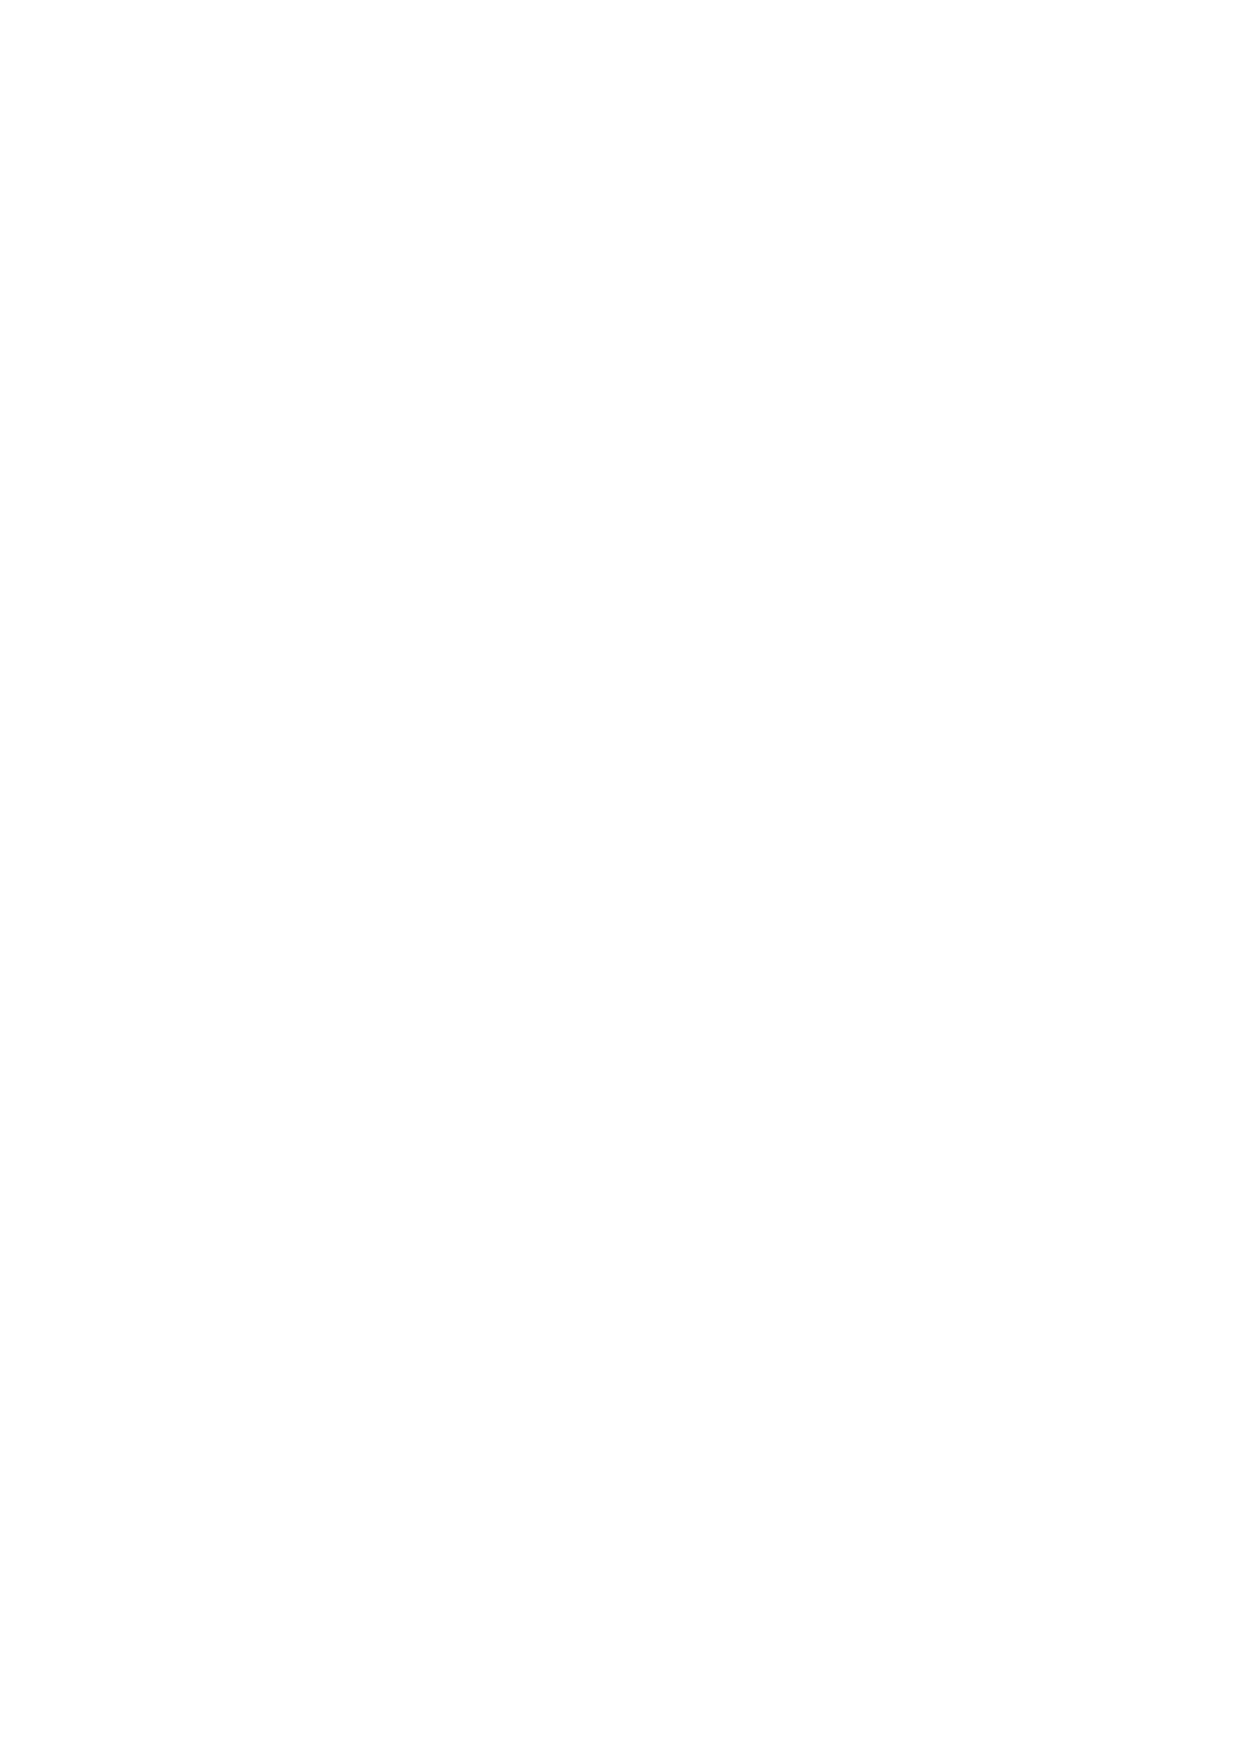
\includepdf{fichacatalografica.pdf}
\end{fichacatalografica}
%
%
% Ou, você poderá também ler os dados da ficha e adicionar no póprio código
% como as palavras-chave, CDU e dimensões do trabalho: 

% ---

% ---
% Inserir folha de aprovação
% ---

% Isto é um exemplo de Folha de aprovação, elemento obrigatório da NBR
% 14724/2011 (seção 4.2.1.3). Você pode utilizar este modelo até a aprovação % do trabalho. Após isso, substitua todo o conteúdo deste arquivo por uma % imagem da página assinada pela banca com o comando abaixo:
%
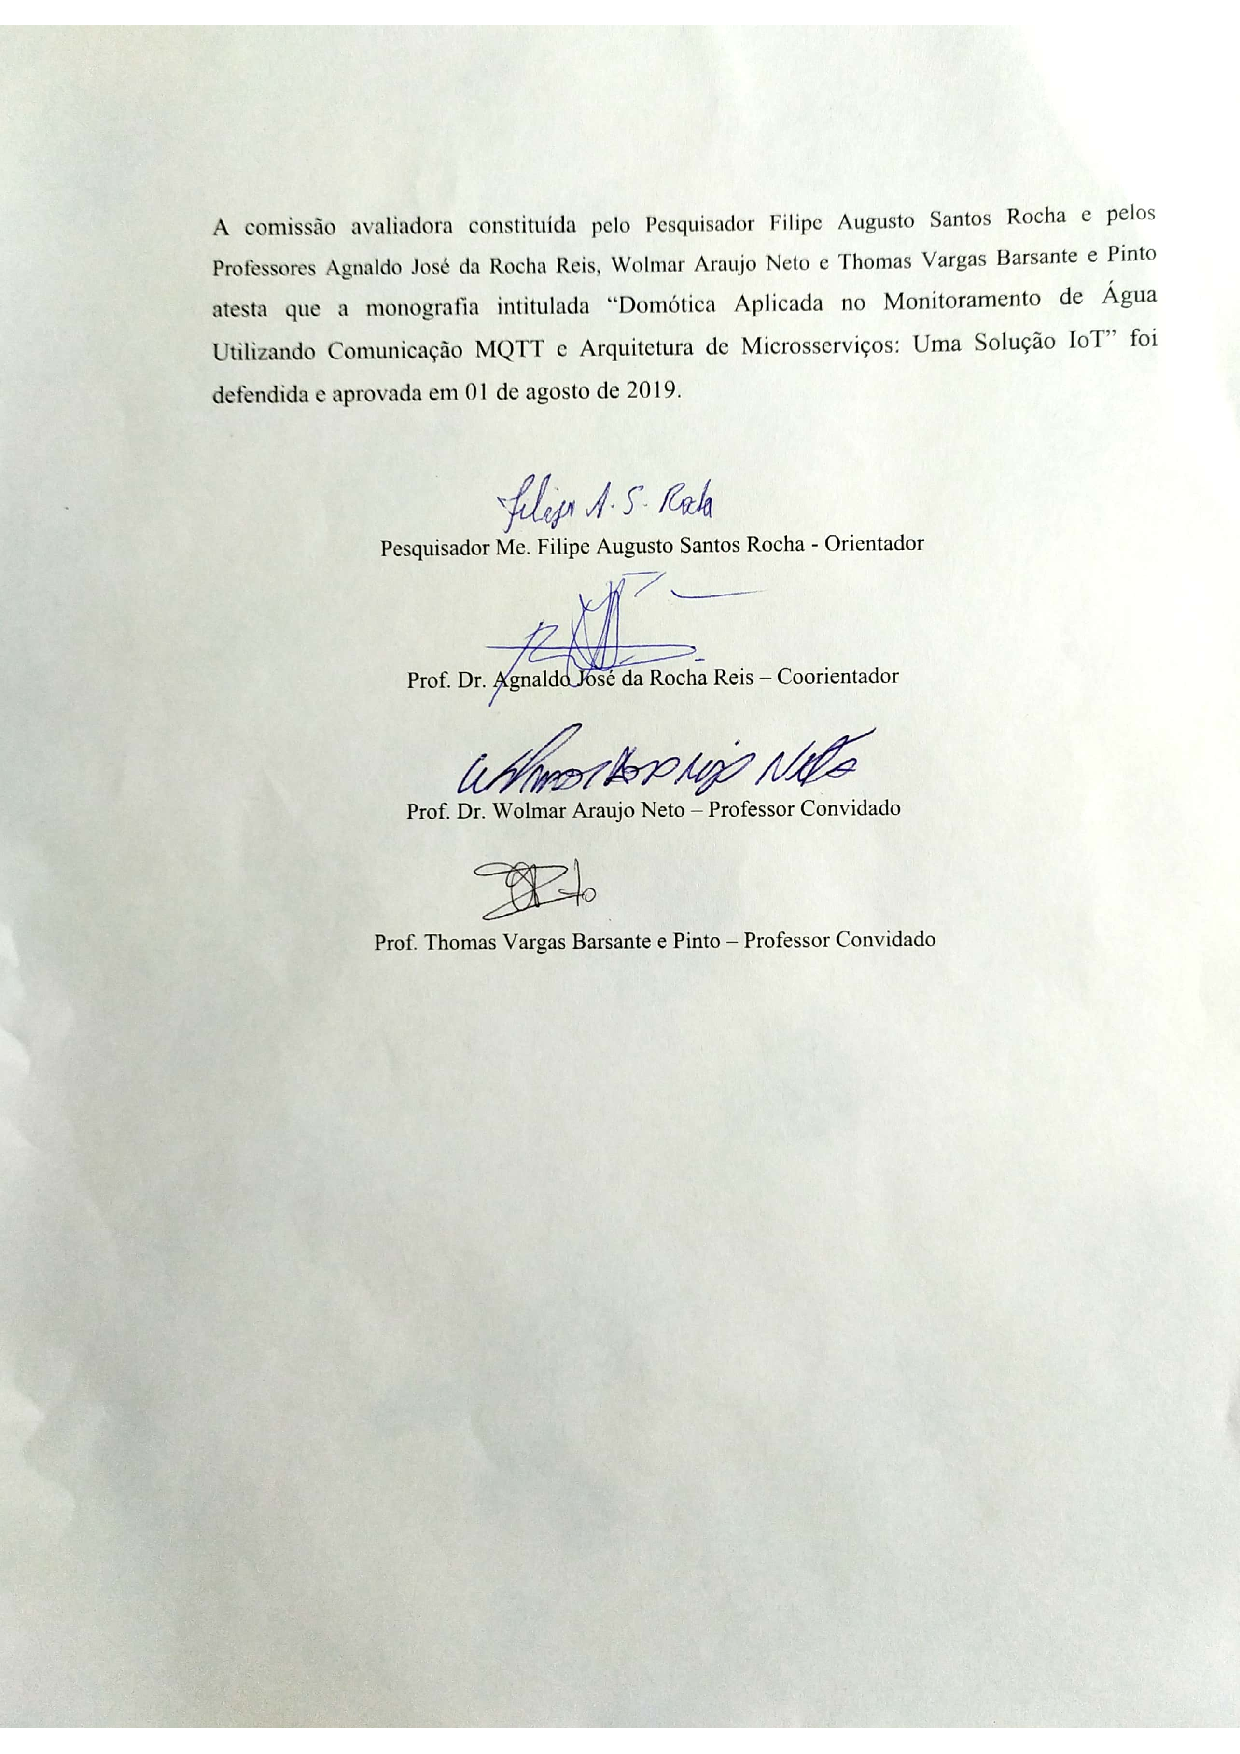
\includepdf{folhadeaprovacao.pdf}
%

% ---

% ---
% Dedicatória
% ---
% \begin{dedicatoria}
%   \vspace*{\fill}
%   \flushright
%   \noindent
%   \textit{ Este trabalho é dedicado às crianças adultas que,\\
%   quando pequenas, sonharam em se tornar cientistas.} \vspace*{\fill}
% \end{dedicatoria}
% ---

% ---
% Agradecimentos
% ---
%\begin{agradecimentos}
%\noindent Os agradecimentos depois de pronto.
%
%\end{agradecimentos}
% ---
% ---
% Epígrafe
% ---
%\begin{epigrafe}
%    \vspace*{\fill}
	%\begin{flushright}
	%	\textit{``Matéria é a parte acidental.'' (Oliver Lodge)}
	%\end{flushright}
%\end{epigrafe}
% ---

% ---
% RESUMOS
% ---

% resumo em português
\setlength{\absparsep}{18pt} % ajusta o espaçamento dos parágrafos do resumo
\begin{resumo}
 \noindent
A finalidade deste trabalho é o desenvolvimento de um software capaz de extrair e reconhecer com precisão os códigos de barras e os números localizados nas etiquetas de identificação dos tarugos originados do processo de Lingotamento Contínuo (LC) de uma siderúrgica. 
%
No processo siderúrgico, o maior problema enfrentado é a mistura de diferentes tipos de aço durante as etapas de fabricação. Portanto, a identificação detalhada de cada umas dessas etapas é essencial. 
%
O projeto foi desenvolvido utilizando técnicas de \textit{Machine Learning} para sua implementação. Foram criados e treinados \textit{datasets} e redes neurais e para detecção dos números e códigos de barras das etiquetas. 
%
Também foi desenvolvido um sistema web com telas para que o usuário tenha uma melhor visualização e gerenciamento dos resultados obtidos pelo sistema de detecção. 
%
Atualmente, a identificação e contagem dos tarugos do estoque são feitas manualmente. 
Devido ao histórico de erros humanos durante o procedimento, foi pensada em uma alternativa para solucionar o problema criando uma aplicação, na qual seria necessária apenas o uso de uma câmera fotográfica.
%
Por fim, o projeto se comportou como o esperado, identificando em média, 99,05\% dos códigos de barras e 91,86\% dos números. 

 \textbf{Palavras-chaves}: aprendizado de máquina, computação da nuvem, IoT, reconhecimento de imagem, código de barras, deep learning, desenvolvimento web.
\end{resumo}

% resumo em inglês
\begin{resumo}[Abstract]
  \begin{otherlanguage*}{english}

 \noindent 
This study highlights a software developed to precisely extract and recognize billet’s identification numbers originated from the Continuous Casting (CC) of a steel mill.
%
This software intends to increase the reliability and automation of this stage of steel production, furthermore make the billets traceable. 
%
This software aims, not only to make billets traceable, but also to increase the reliability and automation at this stage of steel production.
%
One of the main issues in the steel production is the mix of different kinds of steel, therefore a detailed identification of each step becomes crucial, specially before going to the Lamination process, where billets are stocked and pilled up prior to this next step.
%
The identification and count of billets are currently done manually, however due to historical errors caused at this stage an opportunity to improve and automate this process was found. Therefore a simple software application that only requires a digital camera was developed to serve as an alternative solution to this issue in the CC process.

   \vspace{\onelineskip}
 
   \noindent 
   \textbf{Key-words}: machine learning, cloud computing, iot, image recognition, barcode, deep learning, web development.
  \end{otherlanguage*}
\end{resumo}

% resumo em francês 
%\begin{resumo}[Résumé]
% \begin{otherlanguage*}{french}
%    Il s'agit d'un résumé en français.
% 
%   \textbf{Mots-clés}: latex. abntex. publication de textes.
% \end{otherlanguage*}
%\end{resumo}
%
%% resumo em espanhol
%\begin{resumo}[Resumen]
% \begin{otherlanguage*}{spanish}
%   Este es el resumen en español.
%  
%   \textbf{Palabras clave}: latex. abntex. publicación de textos.
% \end{otherlanguage*}
%\end{resumo}
%% ---

% ---
% inserir lista de ilustrações
% ---
\pdfbookmark[0]{\listfigurename}{lof}
\listoffigures*
\cleardoublepage
% ---

% ---
% inserir lista de tabelas
% ---
\pdfbookmark[0]{\listtablename}{lot}
\listoftables*
\cleardoublepage
% ---

% ---
% lista de codigos
% ---
\renewcommand{\lstlistingname}{Código}
\renewcommand{\lstlistlistingname}{Lista de códigos}
\lstlistoflistings
\cleardoublepage
% ---

% ---
%D inserir lista de abreviaturas e siglas
% ---
\begin{siglas}
  \item[CV] \textit{Convertedor}
  \item[MLC] \textit{Máquina de Lingotamento Contínuo}
  \item[JSON] \textit{Javascript Object Notation}
  \item[XML] \textit{Extensible Markup Language}
  \item[VOC] \textit{Visual Object Classes}
  \item[GPU] \textit{Graphics Processing Unit}
  \item[TPU] \textit{Tensor Processing Unit}
  \item[YOLO] \textit{You Only Look Once}
  \item[CNN] \textit{Convolutional Neural Networks}
  \item[R-CNN] \textit{Region - Convolutional Neural Networks}
  \item[ML] \textit{Machine Learning}
  \item[EDA] \textit{Event-Driven Architecture}
  \item[mAP] \textit{Mean Average Precision}
  \item[bbox] \textit{Bounding Box}
  \item[OpenCV] \textit{Open Source Computer Vision}
  \item[HTML] \textit{HyperText Markup Language}
  \item[CSS] \textit{Cascading Style Sheets}
  \item[EJS] \textit{Embedded JavaScript templating}
  \item[HTTP] \textit{Hypertext Transfer Protocol}
  \item[WWW] \textit{World Wide Web}
  \item[W3C] \textit{World Wide Web Consortium}
  \item[FPS] \textit{Frames Per Second}
  
%  \item[RESTful] \textit{Representational State Transfer}
%  \item[API] \textit{Application Programming Interface}
  
\end{siglas}
% ---

% ---
% inserir lista de símbolos
% ---
%\begin{simbolos}
  % \item[$ \Gamma $] Letra grega Gama
  % \item[$ \Lambda $] Lambda
  % \item[$ \zeta $] Letra grega minúscula zeta
  % \item[$ \in $] Pertence
%\end{simbolos}
% ---

% ---
% inserir o sumario
% ---
\pdfbookmark[0]{\contentsname}{toc}
\tableofcontents*
\cleardoublepage
% ---


% ----------------------------------------------------------
% ELEMENTOS TEXTUAIS
% ----------------------------------------------------------
\textual
% ----------------------------------------------------------
% PARTE
% ----------------------------------------------------------
%\part{Preparação da pesquisa}
% ----------------------------------------------------------
%
% ---
% Modelo de capitulo com a introducao, objetivos e estrutura do texto
% ---
% ----------------------------------------------------------
% Introdução (exemplo de capítulo sem numeração, mas presente no Sumário)
% ----------------------------------------------------------
\chapter[Introdução]{Introdução}
%\addcontentsline{toc}{chapter}{Introdução
% ----------------------------------------------------------

 A siderurgia é o ramo da metalurgia que se dedica à fabricação de ferro e aço  através do processamento do minério ferro, sucata, carbono, carvão e fundentes (\textit{e.g.} calcário e dolomita). Existem dois tipos de usinas siderúrgicas: a usina simples, que só utiliza como matéria prima o carvão mineral e a usina integrada, que utiliza tanto o carvão mineral como o carvão vegetal em sua produção (Figura \ref{fig:fluxogramaSiderurgia}).
 
  \begin{figure}[H]
	\centering
	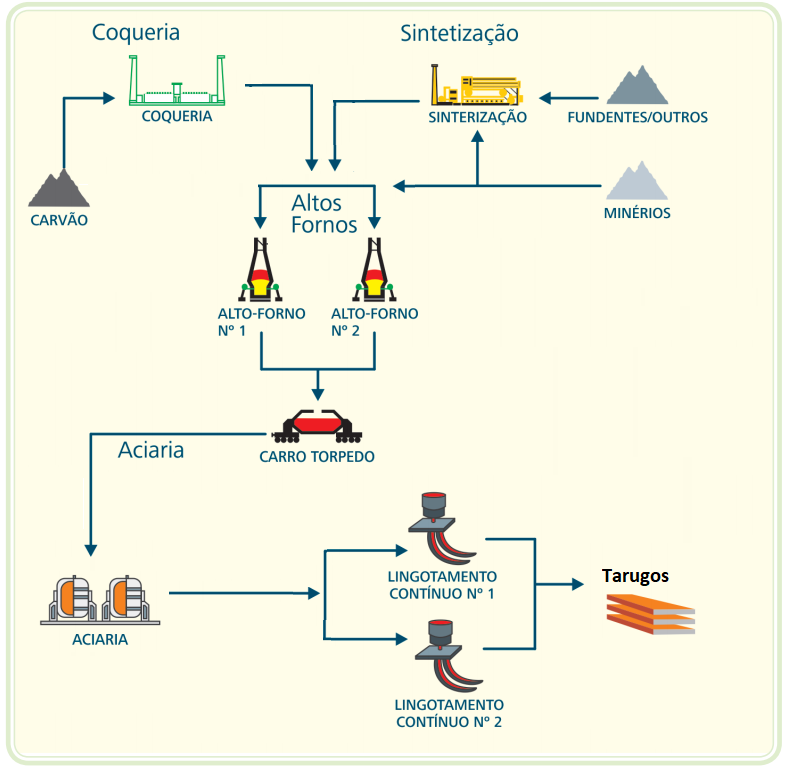
\includegraphics[width=0.6\linewidth]{figuras/Steel/fluxogramaSiderurgia.png}
	\caption{Processo siderúrgico}
	\legend{Fonte: \cite{silva2016siderurgia} }
	\label{fig:fluxogramaSiderurgia}
\end{figure}

 A primeira etapa do processo siderúrgico é a Coqueria. Nela, o minério de ferro é transformado em pelotas através do processo de Pelotização e o carvão mineral é destilado para obtenção do coque.
%
As usinas integradas incluem o processo de Sinterização, cujo intuito é produzir sínter por meio da aglomeração do minério de ferro, fundentes e finos de coque.

 O coque e o sínter são levados aos Alto-Fornos, cuja temperatura média de operação é de 1.500ºC. Dentro dos Alto-Fornos, o ferro se liquefaz e passa a ser chamado de ferro-gusa. Ele é levado à Aciaria por carros torpedos para refinamento através da queima das impurezas. Ainda na Aciaria, a oxidação de elementos como o carbono, silício, fósforo e enxofre transformam o ferro-gusa em aço líquido. Ele é então encaminhado para o Lingotamento Contínuo e, em processo de solidificação, é trabalhado mecanicamente e transformado em produtos como tarugos, bobinas, arames, etc \cite{aco}.

Na usina da Gerdau em Ouro Branco, o processo de lingotamento consiste no despejamento de uma panela com aproximadamente 224 toneladas de aço, a uma temperatura de cerca de 1550ºC, no distribuidor que precede o lingotamento em si como mostra a Figura \ref{fig:processLing}.
%
Este processo pode levar de horas a dias sem interrupção.
%
Cada batelada da panela é chamada de corrida.
%
No final de cada corrida, os tarugos são cortados na máquina Oxicorte, de modo que o tamanho é previamente definido de acordo com a necessidade do cliente, como identificado pelo número 5 na Figura \ref{fig:processLing}

 \begin{figure}[H]
	\centering
	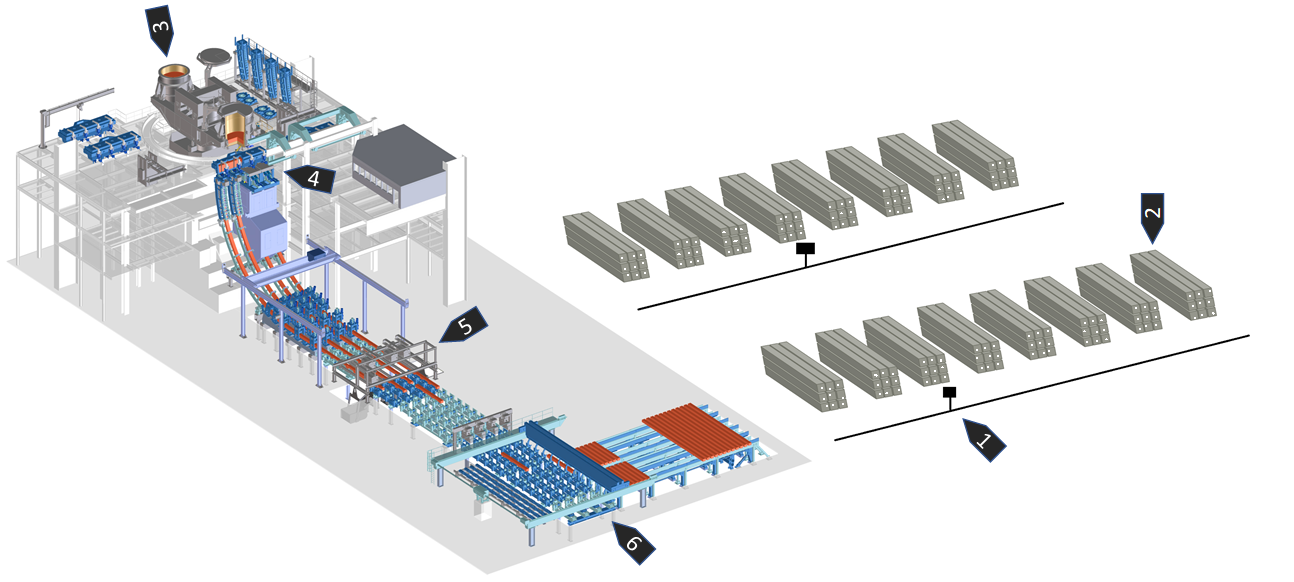
\includegraphics[width=1\linewidth]{figuras/Steel/process.png}
	\caption{Processo de lingotamento Contínuo de Tarugos}
	\legend{Fonte: \cite{freitas2013analise} }
	\begin{tabular}{r@{: }l r@{: }l}
        1 & Câmera Fotográfica & 4 & Molde \\
        2& Pilha de corridas & 5 & Máquina de Oxicorte \\
        3 & Panela de aço& 6 & Transferidor de tarugos \\
    \end{tabular}
	\label{fig:processLing}
\end{figure}

A etapa de solidificação ocorre de fora para dentro do veio
%
\footnote{\textit{Veio} é o nome que se dá ao conjunto formado pelo molde, a máquina Oxicorte e os rolos de extração e endireitadores. Quanto maior o número de veios mais produtiva é da máquina, porém mais complexo se torna seu controle.} 
%
em função do contato com as paredes refrigeradas do molde, aspersão de água em \textit{sprays} e perda de calor por radiação para o ambiente. Essa troca de calor faz com que o aço se solidifique gradativamente criando zonas onde o material pode ser encontrado ao mesmo tempo em seus estados sólido na parte exterior e líquido no interior (Figura \ref{fig:processLingSolid}).

\begin{figure}[H]
	\centering
	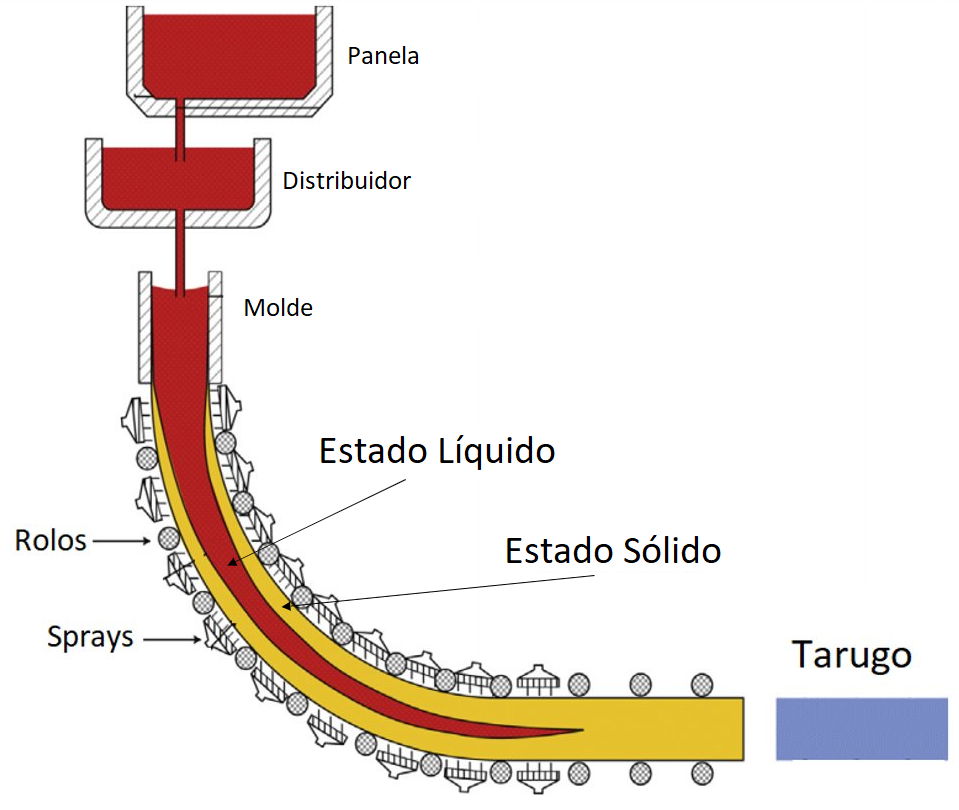
\includegraphics[width=0.6\linewidth]{figuras/Steel/estadoSolidoLiq.png}
	\caption{Estados do aço no processo de lingotamento contínuo}
	\legend{Fonte: \cite{YU201736}}
	\label{fig:processLingSolid}
\end{figure}

Os tamanhos dos cortes são feitos de acordo com a demanda do cliente. O número de tarugos depende do diâmetro das peças que podem ser de 130mm ou 160mm e do comprimento das mesmas que variam de 07 a 14m. Todas as peças de uma mesma corrida têm o mesmo diâmetro e comprimento. Após serem cortados, os tarugos são transportados para o despacho por uma ponte rolante a base de eletroímãs que suportam altas temperaturas e $27$ toneladas de carga (Figura \ref{fig:crane}). 

\begin{figure}[H]
	\centering
	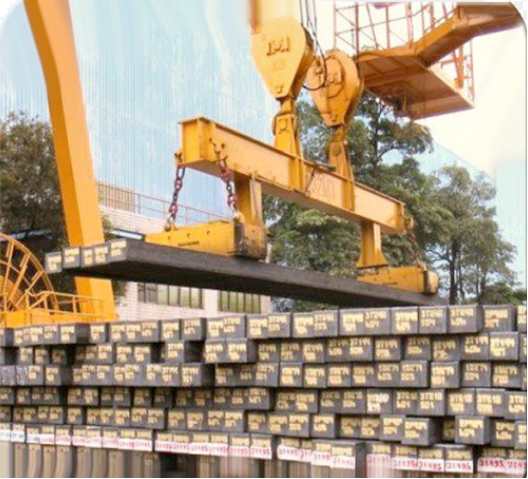
\includegraphics[width=0.5\linewidth]{figuras/Steel/ponte_rolante.png}
	\caption{Ponte Rolante}
	\legend{Fonte: \cite{ponte-rolante})}
	\label{fig:crane}
\end{figure}

Os tarugos vão para a zona de despacho a uma temperatura de aproximadamente 700ºC.
%
Após cerca de 20 horas a temperatura cai para $150~$ºC, adequada para a fixação das etiquetas de identificação dos tarugos.
%
Um jato de água é direcionado aos tarugos para acelerar o resfriamento como mostrado na Figura \ref{fig:despacho} com vazão constante apenas na parte frontal.
%
A eventual injeção de água no centro do tarugo pode empenar a peça, uma vez que a temperatura central do tarugo está mais quente que as extremidades.

Após o tempo necessário, o operador prega as etiquetas utilizando Silicone Acético Transparente, material comprovadamente aderente em altas temperaturas.

\begin{figure}[H]
	\centering
	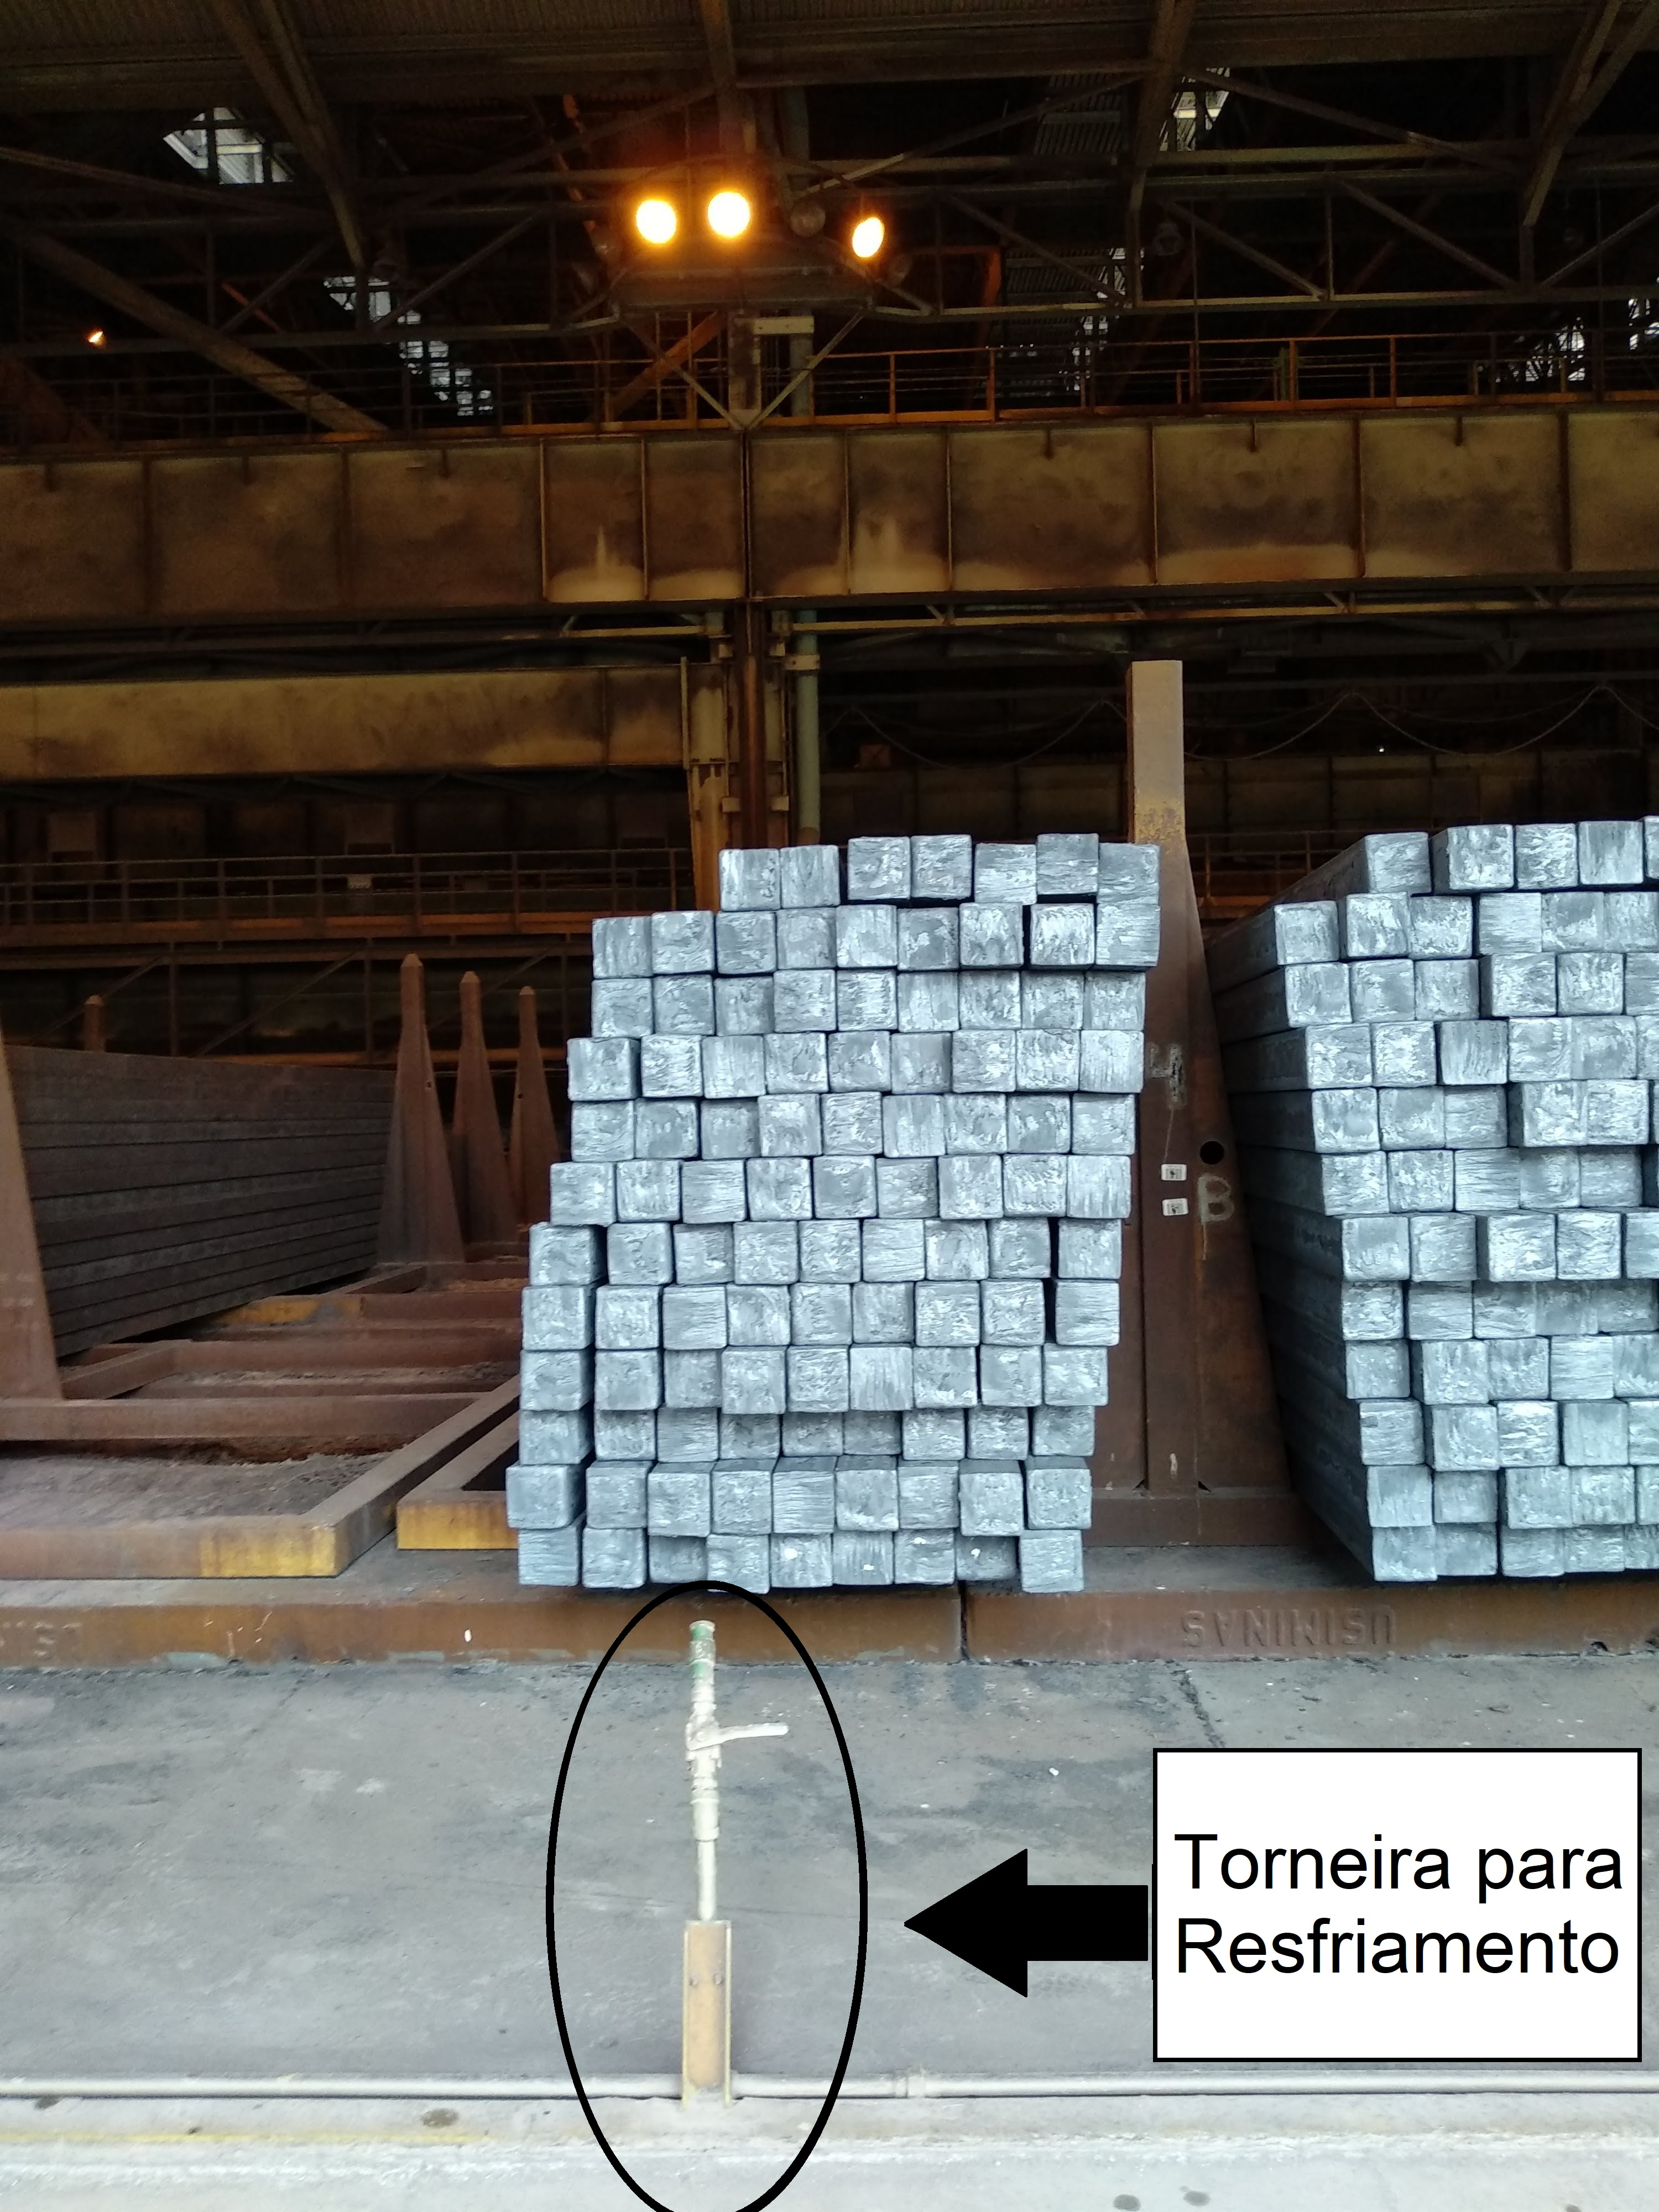
\includegraphics[width=0.5\linewidth]{figuras/Steel/despacho.jpg}
	\caption{Exemplo de Despacho: estoque de uma corrida}
	\label{fig:despacho}
\end{figure}

\begin{figure}[H]
	\centering
	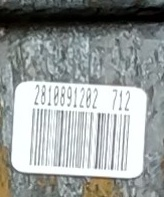
\includegraphics[width=0.25\linewidth]{figuras/Steel/barcode.jpg}
	\caption{Detalhe de uma etiqueta identificadora de um tarugo.} 
	\label{fig:barcode}
\end{figure}

A rotulação é importante pois evita a mistura de aço entre uma corrida e outra, viabiliza a rastreabilidade e identificação do aço em processos posteriores como, por exemplo, na laminação até o cliente final. A tabela \ref{tab:tag} mostra o que cada dígito da etiqueta significa.

\begin{table}[H]
	\centering
	\begin{tabular}{|l|l|}
		\hline
		\rowcolor[HTML]{ECF4FF} 
		\multicolumn{1}{|c|}{\cellcolor[HTML]{ECF4FF}Número} & \multicolumn{1}{c|}{\cellcolor[HTML]{ECF4FF}2810891202 712}\\ \hline
		28 & Número do convertedor que pode ser CV1 (27) ou CV2 (28).\\ \hline
		108912 & Adicionando o convertedor a este número, forma-se o número da corrida no qual: 
    		    \cr & CV2 = 2 e CV1 = 1, temos
    		    \cr & Número da corrida: 2108912\\ \hline
        02 & 02 é a rota que a panela passou no lingotamento. Ou seja, 02 = tarugo.\\ \hline
        712 & Número 7 é o veio que a peça foi lingotada e 12 o número da peça.\\ \hline
	\end{tabular}
	\caption{Significado dos dígitos da etiqueta de rotulação.}
	\label{tab:tag}
\end{table}

O número de identificação da etiqueta pode ser reconhecido pelos dígitos ou pelo código de barras através de um leitor de código de barras à \textit{laser}. Em cada etiqueta, o código de barras e os dígitos acima deste correspondem à mesma sequência numérica. Usualmente, a identificação ou leitura das etiquetas é feita por seres humanos e não por máquinas ou sistemas automáticos. Isto leva aos seguintes problemas:

\begin{enumerate}
	\item O processo é manual e demorado;
	\item O local em que a pilha de peças se encontra é perigoso devido ao fato de, a todo momento, uma ponte rolante estar trabalhando no mesmo local.
\end{enumerate}

\section{Revisão bibliográfica} 

Nesta seção é realizada a pesquisa na literatura a fim de investigar a relevância da automatização do processo de reconhecimento de imagem em indústrias siderúrgicas. Apresenta-se trabalhos semelhantes ao projeto proposto, bem como as dificuldades encontradas durante seus desenvolvimentos. 

Apesar do alto grau adaptativo e cognitivo, a identificação de imagens por uma pessoa pode gerar deficiências no processo por ser totalmente ligado à capacidade e estado do colaborador. O produto final do reconhecimento feito por um operador depende do nível de preparo, treinamento, capacidade visual e concentração, dentre outros fatores. \cite{refbib1} 
%
Além disto, estes parâmetros não são constantes, sofrendo alteração por motivos externos, como por exemplo, a iluminação ou cansaço. \cite{refbib2, refbib3}

No trabalho \citeauthor{ref1}, o autor trata da extração de números de gerenciamento de placas (SMNs) de imagens estáticas capturadas para automação do processo de fabricação de aço. Para impedir a mistura do produto em cada etapa da fabricação de aço, é essencial um sistema de reconhecimento automático das SMNs (Figura \ref{fig:SMN}). Além disso, o algoritmo de extração de SMNs com desempenho robusto é necessário porque afeta seriamente o desempenho de todo o sistema de reconhecimento. Contudo, resultados experimentais mostram que o algoritmo proposto é confiável. 

\begin{figure}[htbp]
	\centering
	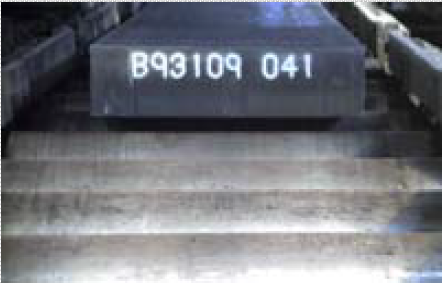
\includegraphics[width=0.5\linewidth]{figuras/Steel/SMN.png}
	\caption{Número de gerenciamento de placa}
	\label{fig:SMN}
\end{figure}


Em \citeonline{ref2}, os autores desenvolvem um sistema de reconhecimento em tempo real para caracteres gravados no material de placas e tarugos na planta de ferro fundido. 
%
Os tarugos normalmente são misturados no despacho, de modo que suas identificações são dificilmente tratáveis. Os caracteres dessa imagem do material podem ser marcados pelo uso de três tipos de métodos, como máquina de marcação automática, placa de marcação de modelo e escrita à mão. Para a aplicação do algoritmo de reconhecimento, desenvolveu-se um sistema de visão e instalou-se na linha de produção de placas e tarugos da planta de aço-ferro. Por meio do teste, confirmou-se que o sistema apresentou-se bom desempenho e alta taxa de reconhecimento: 97,6\% para placas e 98,6\% para tarugos.

\section{Objetivos} 

O objetivo deste trabalho é desenvolver um sistema automático para o reconhecimento de etiquetas identificadoras em tarugos e uma interface para que o operador realize as conferências. 

Por meio de uma foto, o sistema será capaz de contar o número de etiquetas, identificar o código de barras e os números acima dele. Será criada uma aplicação web para que seja gerado, de forma automática, um relatório detalhado e facilitar a conferência por parte do operador.

\section{Organização do trabalho}

O presente trabalho está organizado em 4 capítulos. O atual apresenta o problema, possíveis soluções, e os objetivos propostos.
%
O Capítulo 2 apresenta a estrutura geral dos sistemas, das linguagens de programação, das bibliotecas, dos métodos e dos \textit{softwares} utilizados no projeto.
%
No Capítulo 3 são apresentados o desenvolvimento e os resultados deste trabalho. Explica-se também os experimentos realizados e códigos implementados.
%
No Capítulo 4 são abordadas as considerações finais do trabalho.
% ---
% Capitulo com exemplos de comandos inseridos de arquivo externo 
% ---
%\include{capitulos/capitulo-abntex2-modelo-include-comandos}
% ---
% ----------------------------------------------------------
% PARTE
% ----------------------------------------------------------
%\part{Materiais e metodos}
% ----------------------------------------------------------
% ---
% Capitulo de revisão de literatura
% ---

% ----------------------------------------------------------
%\part{Metodologia}
% ----------------------------------------------------------
% ---
% Capitulo de metodologia
% ---
 \chapter{Metodologia}
 
Este capítulo apresenta a estrutura geral do sistema, que se divide em duas partes. A primeira parte consiste no \textit{backend} desenvolvido em Python com o objetivo de reconhecer as etiquetas utilizando técnicas de \textit{Machine Learning}. A segunda parte consiste na aplicação web, desenvolvida em Node.JS, responsável pela visualização e gerenciamento do sistema através de relatórios e telas.

A validação do projeto será feita através de um sistema que seja capaz de identificar números localizados em etiquetas em uma única imagem.

%------------------------------------------------

\section{Visão geral do sistema} \label{sec:funcionamento}

Esta seção descreve as características operacionais do sistema, assim como os resultados esperados. O fluxo geral do sistema pode ser visualizado na Figura \ref{fig:arqgeral}.

\begin{figure}[htbp]
	\centering
	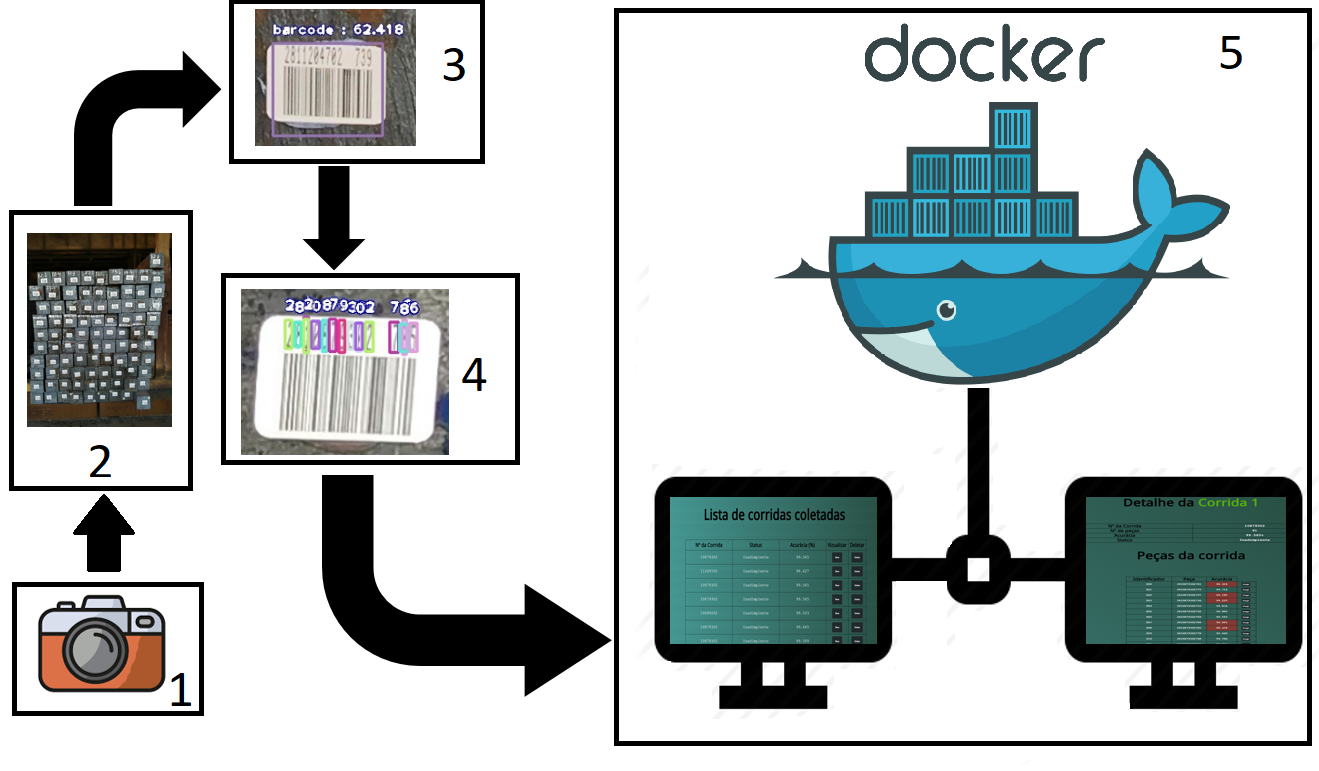
\includegraphics[width=1\linewidth]{capitulos/FluxoDoProjeto.png}
	\caption{Arquitetura geral do projeto.}
	\begin{tabular}{r@{: }l r@{: }l}
    1 & Câmera Fotográfica & 4 & Identificação de números \\
    2& Foto das peças da corrida & 5 & Aplicação WEB \\
    3 & Identificação dos códigos de  barra
    \end{tabular}
	\label{fig:arqgeral}
\end{figure}

Em suma, o processo será realizado em diversos passos sequenciais. Será iniciado ao se fotografar as peças de uma corrida no setor de despacho utilizando uma câmera digital. A fotografia vai automaticamente para o sistema e a partir dela dá-se início reconhecimento da imagem. O código de barras de cada tarugo é detectado como um bloco e, em seguida, os números que estão acima de cada um dos blocos é identificado.Esse processo é chamado de corrida. 

A corrida é salva em um banco de dados e exibidas através de telas para que o usuário possa validá-las.

%------------------------------------------------

\section{Backend em Python} \label{sec:backend}

Para realizar o experimento é necessário treinar um modelo de rede neural que seja capaz de reconhecer código de barras e algarismos. Para isso, são efetuadas três etapas. Primeiro é coletado o maior número possível de imagens dos códigos de barras. Em seguida, é gerado um \textit{dataset} com as características dessas imagens juntamente com a classe em que pertence. Então, é possível realizar a configuração e treinamento da rede neural. Por fim é calculada a acurácia, mediante imagens de teste, do modelo que obteve a melhor performance no treinamento.

A linguagem de programação Python para implementação do sistema de Machine Learning foi prioritariamente escolhida devido à grande comunidade existente da linguagem, ao grande número de bibliotecas de análise de dados disponíveis e ao fato da ferramenta Google Colab utilizá-lo, permitindo o processamento que não seria possível em um computador de baixa performance.

%------------------------------------------------

\subsubsection*{Python}

Python é uma linguagem de programação interpretada\footnote{Linguagem interpretada é uma linguagem de programação em que o código fonte é executado por um programa de computador chamado interpretador, que em seguida é executado pelo sistema operacional ou processador.} de alto nível, ou seja, com um nível de abstração relativamente elevado e de uso geral. Sua abordagem orientada a objetos tem a finalidade de ajudar os programadores a escrever código para projetos de pequena e grande escala.

O Python suporta vários paradigmas de programação, incluindo programação estruturada (principalmente processual), orientada a objetos e funcional.

Os interpretadores de Python estão disponíveis para diversos sistemas operacionais. Uma organização sem fins lucrativos, a Python Software Foundation, gerencia e direciona recursos para o desenvolvimento do Python. \cite{van2007python}

%------------------------------------------------

\subsection{Preparação do dataset}

Como o escopo do trabalho não contempla a automatizacão da recuperação de informações de \textit{websites} públicos, foi disponibilizado um repositório com imagens. Esse
repositório possui 500 imagens e foi disponibilizado pelo laboratório Applied Recognition Technology Laboratory. As imagens se tratam de diferentes tipos de códigos de barras.\cite{Arte-Lab}

\begin{figure}[htbp]
	\centering
	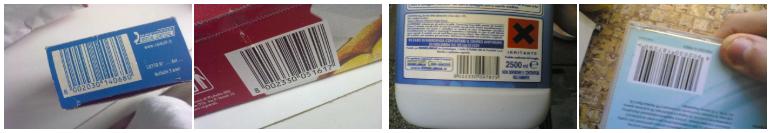
\includegraphics[width=1\linewidth]{figuras/MachineLearning/barcodes.png}
	\caption{Dataset dos código de barras}
	\label{fig:datasetBarcode}
\end{figure}

Para o treinamento de um modelo de rede neural com alta taxa de acerto é ideal que se tenha o maior número possível de imagens no \textit{dataset}. Para isso foi utilizado o método de \textit{Data Augmentation}.  

%------------------------------------------------

\subsubsection*{\textit{Data Augmentation}}\label{sec:dataAugm}

\textit{Data Augmentation} é o processo de aumentar a quantidade e a diversidade de dados de forma sintética. A partir uma imagem, ele pode gerar mais imagens semelhantes através de vários métodos como girar um ângulo qualquer, embaçar a imagem fazendo com que ela perca o brilho ou até mesmo ofuscando-a, entre outros para que possa aumentar o tamanho do \textit{dataset}.

Mesmo quando os dados são de qualidade inferior como, por exemplo, imagens não nítidas, os algoritmos de ML podem ter um desempenho melhor, desde que dados úteis possam ser extraídos pelo modelo do conjunto de dados original. Por exemplo, os modelos de conversão de texto em fala e em texto melhoraram devido ao lançamento de um corpus\footnote{Um corpus pode ser entendido como uma coleção de porções de texto selecionadas de acordo com um conjunto de critérios para representar, tanto quanto possível, uma determinada língua \cite{sinclair2005corpus}} de trilhões de palavras pelo Google \cite{halevy2009unreasonable}. Esse resultado ocorre apesar dos dados serem coletados de páginas da web não filtradas e conter muitos erros.\cite{dataAug}

O Código \ref{cod:dataaug} abaixo mostra o momento em que é definido o tipo de ação que será feita em cada foto, como rotacionar em um ângulo aleatório, inserir ruído na imagem e girar horizontalmente. O método também possibilita escolher a quantidade de imagens que será gerada, neste caso, 1000 imagens.

\begin{lstlisting}[caption=Exemplo de código do método \textit{data augmentation}, label=cod:dataaug][H]
 num_files_desired = 1000
 available_transformations = {
                                'rotate': random_rotation,
                                'noise': random_noise,
                                'horizontal_flip': horizontal_flip
                             }
\end{lstlisting}

%------------------------------------------------

\subsection{Anotações das imagens}

Após ter criado o \textit{dataset}, as anotações das imagens geradas são feitas. Isso quer dizer que é criado um arquivo que contenha as posições dos pixels da \textit{Bounding Box} que engloba o objeto na imagem. Um dos formatos mais conhecidos é o Pascal VOC. O formato VOC do Pascal utiliza arquivos XML para armazenar as informações sobre os objetos anotados nas imagens. Para que seja possível gerar tais arquivos mais facilmente, foi utilizado o software LabelImg.

%------------------------------------------------

\subsubsection*{\textit{Bounding Box}}

A \textit{Bounding Box}(bbox) (Figura \ref{fig:boundingBox}) é um dos métodos de anotação de imagem mais populares usados em \textit{Machine Learning} e em \textit{Deep Learning}.

As bbox são caixas retangulares que podem ser determinadas pelo recorte da imagem baseado nas coordenadas das extremidades. Com exemplo, as bbox do cachorro e do gato da Figura \ref{fig:boundingBox} são definidas com base nas informações de coordenadas da imagem superior. \cite{allDeep}

\begin{figure}[H]
		\centering
		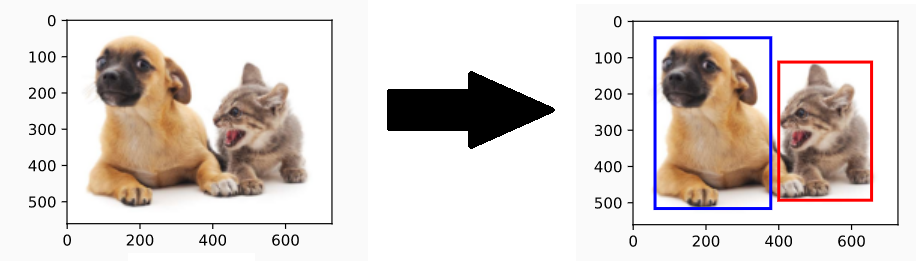
\includegraphics[scale=0.6]{figuras/MachineLearning/catDog.png}
		\caption{Execução de \textit{Bounding Boxes}.}
		\legend{Fonte: \cite{133Ob9905723:online})}
		\label{fig:boundingBox}
\end{figure}

O código \ref{cod:bbox} refere-se à posição das \textit{Bounding Boxes} do cachorro e do gato na imagem, respectivamente.

\begin{lstlisting}[caption=Posições de X e Y nas \textit{Bounding Boxes}, label=cod:bbox]
         dog_bbox, cat_bbox = [60, 45, 378, 516], [400, 112, 655, 493]
\end{lstlisting}

%------------------------------------------------

\subsubsection*{LabelImg}\label{sub:LabelImg}

O LabelImg (Figura \ref{fig:labelimg}) é uma ferramenta \textit{open source} de anotação de imagem gráfica escrita em Python. As anotações são salvas em arquivos XML no formato PASCAL VOC (Código \ref{cod:XML}), o formato usado pelo ImageNet. Além disso, também suporta o formato YOLO que é utilizado no presente projeto. \cite{labelimg}

O software em questão permite que as bbox sejam circuladas englobando o objeto de interesse nas imagens e criando automaticamente um arquivo XML com todas as especificações necessárias.

Utiliza-se o LabelImg para formar o \textit{dataset} que é usado para testar desempenho do algoritmo. Obter dados suficientes para realizar o experimento costuma ser uma dificuldade visto que é necessário um grande volume. Os \textit{datasets open source} ajudam a resolver esta questão ao disponibilizar diversos conjuntos de dados. Alguns \textit{datasets} comumente usados na visão computacional são os seguintes:

\begin{figure}[htbp]
	\centering
	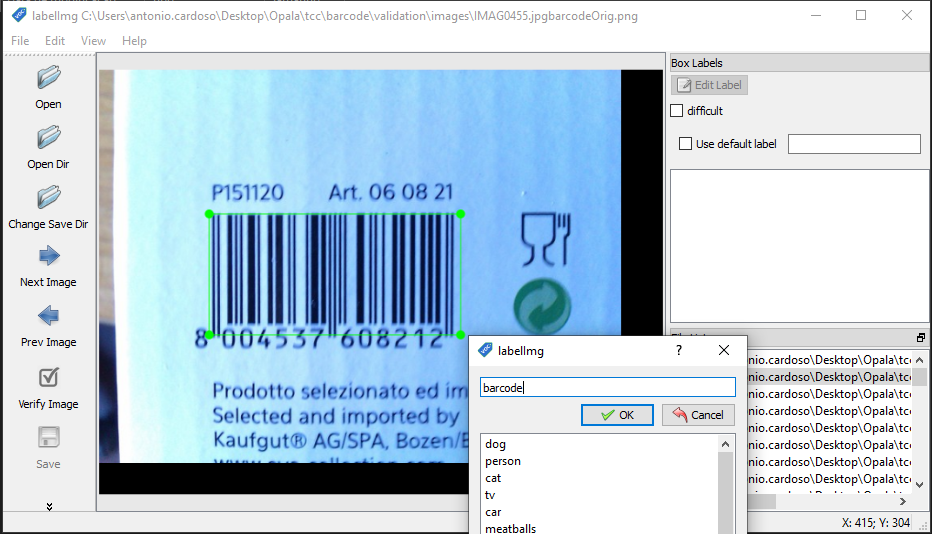
\includegraphics[width=0.9\linewidth]{figuras/MachineLearning/labelimg.png}
	\caption{Procedimento de anotações das \textit{bounding boxes}}
	\label{fig:labelimg}
\end{figure}

\begin{lstlisting}[caption=Arquivo XML gerado pelo LabelImg, label=cod:XML]
<annotation>
	<folder>images</folder>
	<filename>05102009081.jpgbarcodeOrig.png</filename>
	<path>C:\Users\antonio.cardoso\Desktop\tcc\barcode\train\images\05102009081.jpgbarcodeOrig.png</path>
	<source>
		<database>Unknown</database>
	</source>
	<size>
		<width>640</width>
		<height>480</height>
		<depth>3</depth>
	</size>
	<segmented>0</segmented>
	<object>
		<name>barcode</name>
		<pose>Unspecified</pose>
		<truncated>0</truncated>
		<difficult>0</difficult>
		<bndbox>
			<xmin>105</xmin>
			<ymin>63</ymin>
			<xmax>536</xmax>
			<ymax>454</ymax>
		</bndbox>
	</object>
</annotation>
\end{lstlisting}

O ImageNet \textit{dataset} \cite{deng2009imagenet} possui mais de 14 milhões de imagens, cobrindo mais de 20.000 categorias. Existem mais de um milhão de imagens com anotações explícitas de classe e de locais de objetos na imagem. O conjunto de dados ImageNet é um dos mais usados no campo da \textit{Deep Learning} por ser detalhado e de uso intuitivo. \cite{zhou2017application}

\subsubsection*{Pascal VOC}
O Pascal VOC é uma coleção de \textit{datasets} também utilizada para o desenvolvimento deste trabalho. Fornece conjuntos de dados de imagem padronizados para reconhecimento de classe de objetos, além de ferramentas para acessar as anotações.O conjunto de dados não é atualizado desde 2012, porém é de boa qualidade e permite a avaliação e comparação de diferentes métodos. \cite{zhou2017application, everingham2010pascal}.

%-------------

\subsection{Separação do Conjunto de Teste}

Os passos seguintes às anotações das imagens são a separação do conjunto de teste e posteriormente o treinamento do modelo de rede neural. Para a separação, cria-se uma pasta chamada "barcodes" e dentro dela, outras duas pastas de nomes \textbf{train} e \textbf{validation}.

Nenhuma imagem da pasta "train" (conjunto de treinamento) pode estar presente dentro da pasta "validation" (conjunto de validação). O \textit{dataset} de testes tem uma amostra menor que o conjunto de treinamento, cerca de 25\% do total das imagens.

A estrutura da pasta do \textit{dataset} de \textit{barcodes} pode ser visualizada a seguir:

\begin{figure}[H]
	\centering
	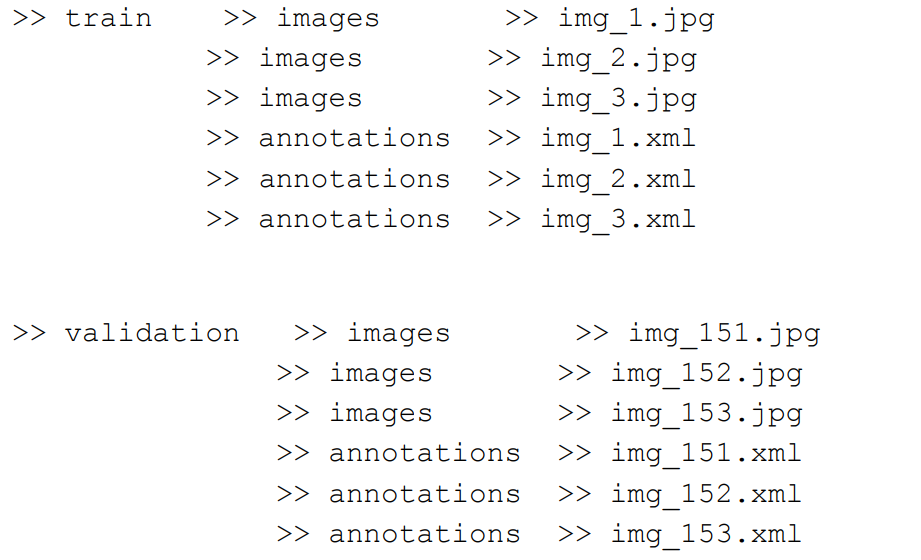
\includegraphics[width=0.5\linewidth]{figuras/MachineLearning/foldersDataset.png}
	\caption{Estrutura de pastas do \textit{dataset} de barcodes}
	\label{fig:labelimg}
\end{figure}

Ou seja, para cada imagem, há um arquivo XML com as anotações registradas pelo Labelimg. A etapa é o treinamento do modelo. Para tanto é necessário a compreensão da infraestrutura e bibliotecas utilizadas no projeto.

%------------------------------------------------

\subsection{Infraestrutura}

Com o intuito de acelerar o processo, foi utilizado um software online chamado Google Colaboratory que tem disponibilidade de configuração com GPU para o treinamento. 

%------------------------------------------------

\subsubsection{Google Colaboratory}
O Google Colaboratory, mais conhecido como "Google Colab" ou simplesmente "Colab", é um projeto de pesquisa para criar protótipos de modelos de \textit{Machine Learning} em poderosas opções de \textit{hardware}, como GPUs e TPUs. Fornece um ambiente de notebook Jupyter sem servidor para desenvolvimento interativo. O Google Colab é gratuito para usar como outros produtos do G Suite, ferramenta corporativa do Google. \cite{colabdetail}
 
Características e Funcionalidades do Google Colab:

\begin{itemize}
    \item Suporte para Python 2.7 e Python 3.6;
    \item Aceleração de GPU;
    \item Bibliotecas pré-instaladas: diversas bibliotecas Python, como TensorFlow, Scikit-learn, Matplotlib etc.
    \item Recurso de colaboração: permite que os desenvolvedores usem e compartilhem o Jupyter notebook entre si sem precisar baixar, instalar ou executar qualquer coisa que não seja um navegador;
    \item Suporta comandos \textit{bash};
    \item Os notebooks do Google Colab são armazenados no drive.
\end{itemize}

\begin{figure}[H]
		\centering
		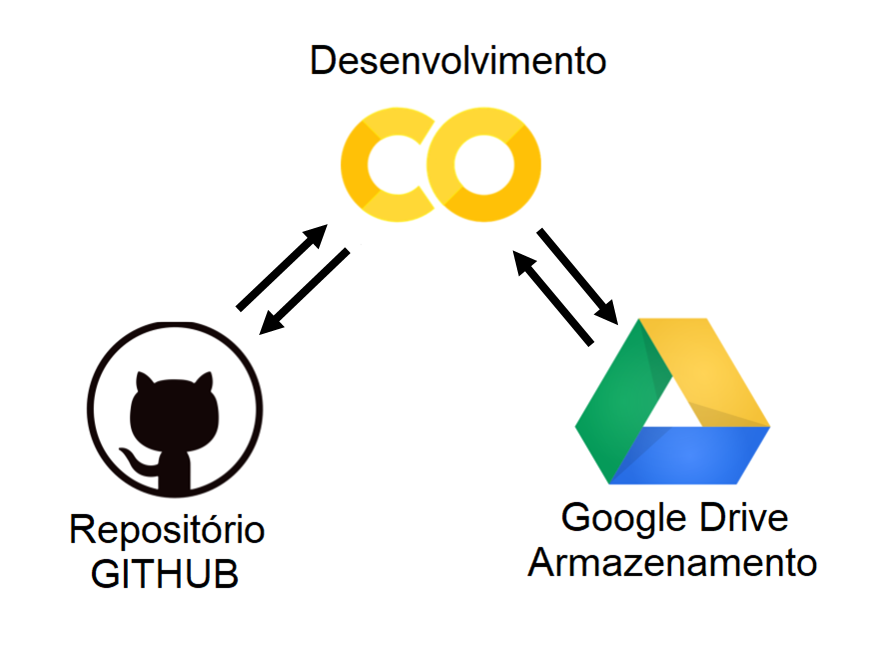
\includegraphics[scale=0.4]{figuras/MachineLearning/colabGithub.png}
		\caption{Utilização do Colab, Drive e Github}
		\label{fig:colabGithub}
\end{figure}

O Google Colab se integra facilmente ao Google Drive, o que o torna uma opção natural para espaço de armazenamento dos dados e modelos. Porém há também outras opções de hospedagem de código, como na plataforma Github, escolhida para este trabalho.

\subsection{Blibliotecas utilizadas}

Todo o código foi implementado utilizando a linguagem de programacão Python, e as seguintes bibliotecas foram utilizadas:

%------------------------------------------------

\subsubsection{TensorFlow}

O TensorFlow é uma biblioteca Python de código aberto para implementar algoritmos de \textit{Machine Learning}. Um código utilizando o TensorFlow pode ser executado com pouca ou nenhuma alteração em uma ampla variedade de sistemas heterogêneos, desde dispositivos móveis como telefones e tablets até sistemas distribuídos em larga escala de centenas de máquinas e milhares de dispositivos computacionais, como placas de GPU.

O sistema é flexível e tem sido usado para conduzir pesquisas e implantar sistemas de aprendizado de máquina na produção em mais de uma dúzia de áreas da ciência da computação e outros campos, incluindo reconhecimento de fala, visão computacional, robótica, recuperação de informações, processamento de idiomas, extração de informações geográficas e descoberta computacional de drogas. \cite{abadi2016tensorflow}

Vários serviços do Google uilizam o TensorFlow em sua produção, foi lançado como um projeto de código aberto e tornou-se amplamente utilizado para pesquisa de ML.\cite{199317}

%------------------------------------------------

\subsubsection{Scikit-Image}

O Scikit-image, também conhecido como Skimage, é uma biblioteca de processamento de imagens que implementa algoritmos e utilitários para uso em aplicações de pesquisa, educação e indústria. É lançado sob a licença liberal de código aberto Modified BSD, fornece uma API bem documentada na linguagem de programação Python e é desenvolvido por uma equipe internacional ativa de colaboradores.

O objetivo do scikit-image é fornecer uma biblioteca de alta qualidade de ferramentas poderosas e diversas de processamento de imagens, gratuitas e sem restrições. Esses princípios são a base para as práticas de desenvolvimento na comunidade de imagens scikit.\cite{skimage}

%------------------------------------------------

\subsubsection{ImageAI}

ImageAI é uma biblioteca python de código aberto criada para capacitar os desenvolvedores a criar aplicativos e sistemas com recursos independentes de \textit{Deep Learning} e \textit{Computer Vision} usando poucas linhas de código.

A biblioteca ImageAI suporta previsão e treinamento de imagens usando 4 algoritmos diferentes de \textit{Machine Learning} treinados no conjunto de dados ImageNet-1000. O ImageAI também suporta detecção de objetos, detecção de vídeo e rastreamento de objetos usando RetinaNet, YOLOv3 e TinyYOLOv3 treinados no conjunto de dados COCO e PASCAL VOC.\cite{ImageAI}

Neste trabalho será utilizada uma classe da biblioteca ImageAI chamada \textit{Custom Detection Model Training}, possibilitando o treinamento do meu próprio modelo de detecção de objetos utilizando a arquitetura da YOLOv3.

%------------------------------------------------

\subsubsection{OpenCV}

O OpenCV (Open Source Computer Vision) é uma biblioteca de \textit{open source} e \textit{cross-plataform} (Multiplataforma) que contém mais de 500 algoritmos otimizados para análise de imagem e vídeo. Desde sua introdução em 1999, ele foi amplamente adotado como a principal ferramenta de desenvolvimento pela comunidade de pesquisadores e desenvolvedores em visão computacional.\cite{opencv}

%------------------------------------------------

\subsection{Treinamento dos modelos}

Após gerado o conjunto de dados, é possível trabalhar no treinamento do modelo da rede neural. Para isso será utilizado o \textit{framework} TensorFlow destinado à \textit{Deep Learning}. Também será utilizado uma rede neural pré-treinada chamada YoloV3, escrita em Python que fará uso das funções disponibilizadas pela biblioteca ImageAI . Assim realizando o treinamento até atingir um valor aceitável de acerto no conjunto de teste. 

Através do modelo da rede Yolov3, treinaremos mais dois novos modelos de redes neurais:
\begin{itemize}
    \item Modelo de rede neural para reconhecimento de \textit{barcodes};
    \item Modelo de rede neural para reconhecimento de algarismos numéricos;
\end{itemize}

O resultado do treinamento serão arquivos no formato .h5\footnote{Um arquivo H5 é um arquivo de dados salvo no formato \textit{Hierarchical Data Format}(HDF). Contém conjuntos multidimensionais de dados científicos.} representando o modelo que serão avaliados através da melhor acurácia\footnote{Indica uma performance geral do modelo. Dentre todas as classificações, quantas o modelo classificou corretamente;} e utilizados posteriormente.

%------------------------------------------------

\subsubsection*{YOLOv3}\label{sub:Yolov3}

A rede neural YOLOv3 evoluiu de YOLO e YOLO-V2 \cite{redmon2018yolov3}. Quando comparado com a rede Faster R-CNN, a mais eficiente das CNNs quando, a YOLO transforma o problema de detecção em um problema de regressão, em que a informação tem um significado numérico resultante de alguma previsão na imagem. Isto não requer uma região da proposta e gera coordenadas e probabilidades de \textit{bounding boxes} (\textit{bbox}) de cada classe diretamente por meio de regressão. Isso aumenta consideravelmente a velocidade de detecção em comparação com o Faster R-CNN.\cite{yolov3_apple}

O YOLO é a frequência mais rápida (45 FPS) do que outros algoritmos de detecção de objetos \cite{yolov3RealTime}. Comparando a rede Faster R-CNN com a  R-CNN, a velocidade do treinamento  é 9 vezes mais rápida e a velocidade do teste é 213 vezes mais rápida. \cite{7960069}

O YOLO impõe fortes restrições espaciais nas previsões de \textit{bbox}, pois cada célula da \textit{grid} prevê apenas duas \textit{box} e pode ter apenas uma classe. Essa restrição espacial limita o número de objetos próximos que o modelo pode prever. O modelo luta com pequenos objetos que aparecem em grupos, como por exemplo, bandos de pássaros. \cite{yolov3RealTime}

\begin{figure}[htbp]
		\centering
		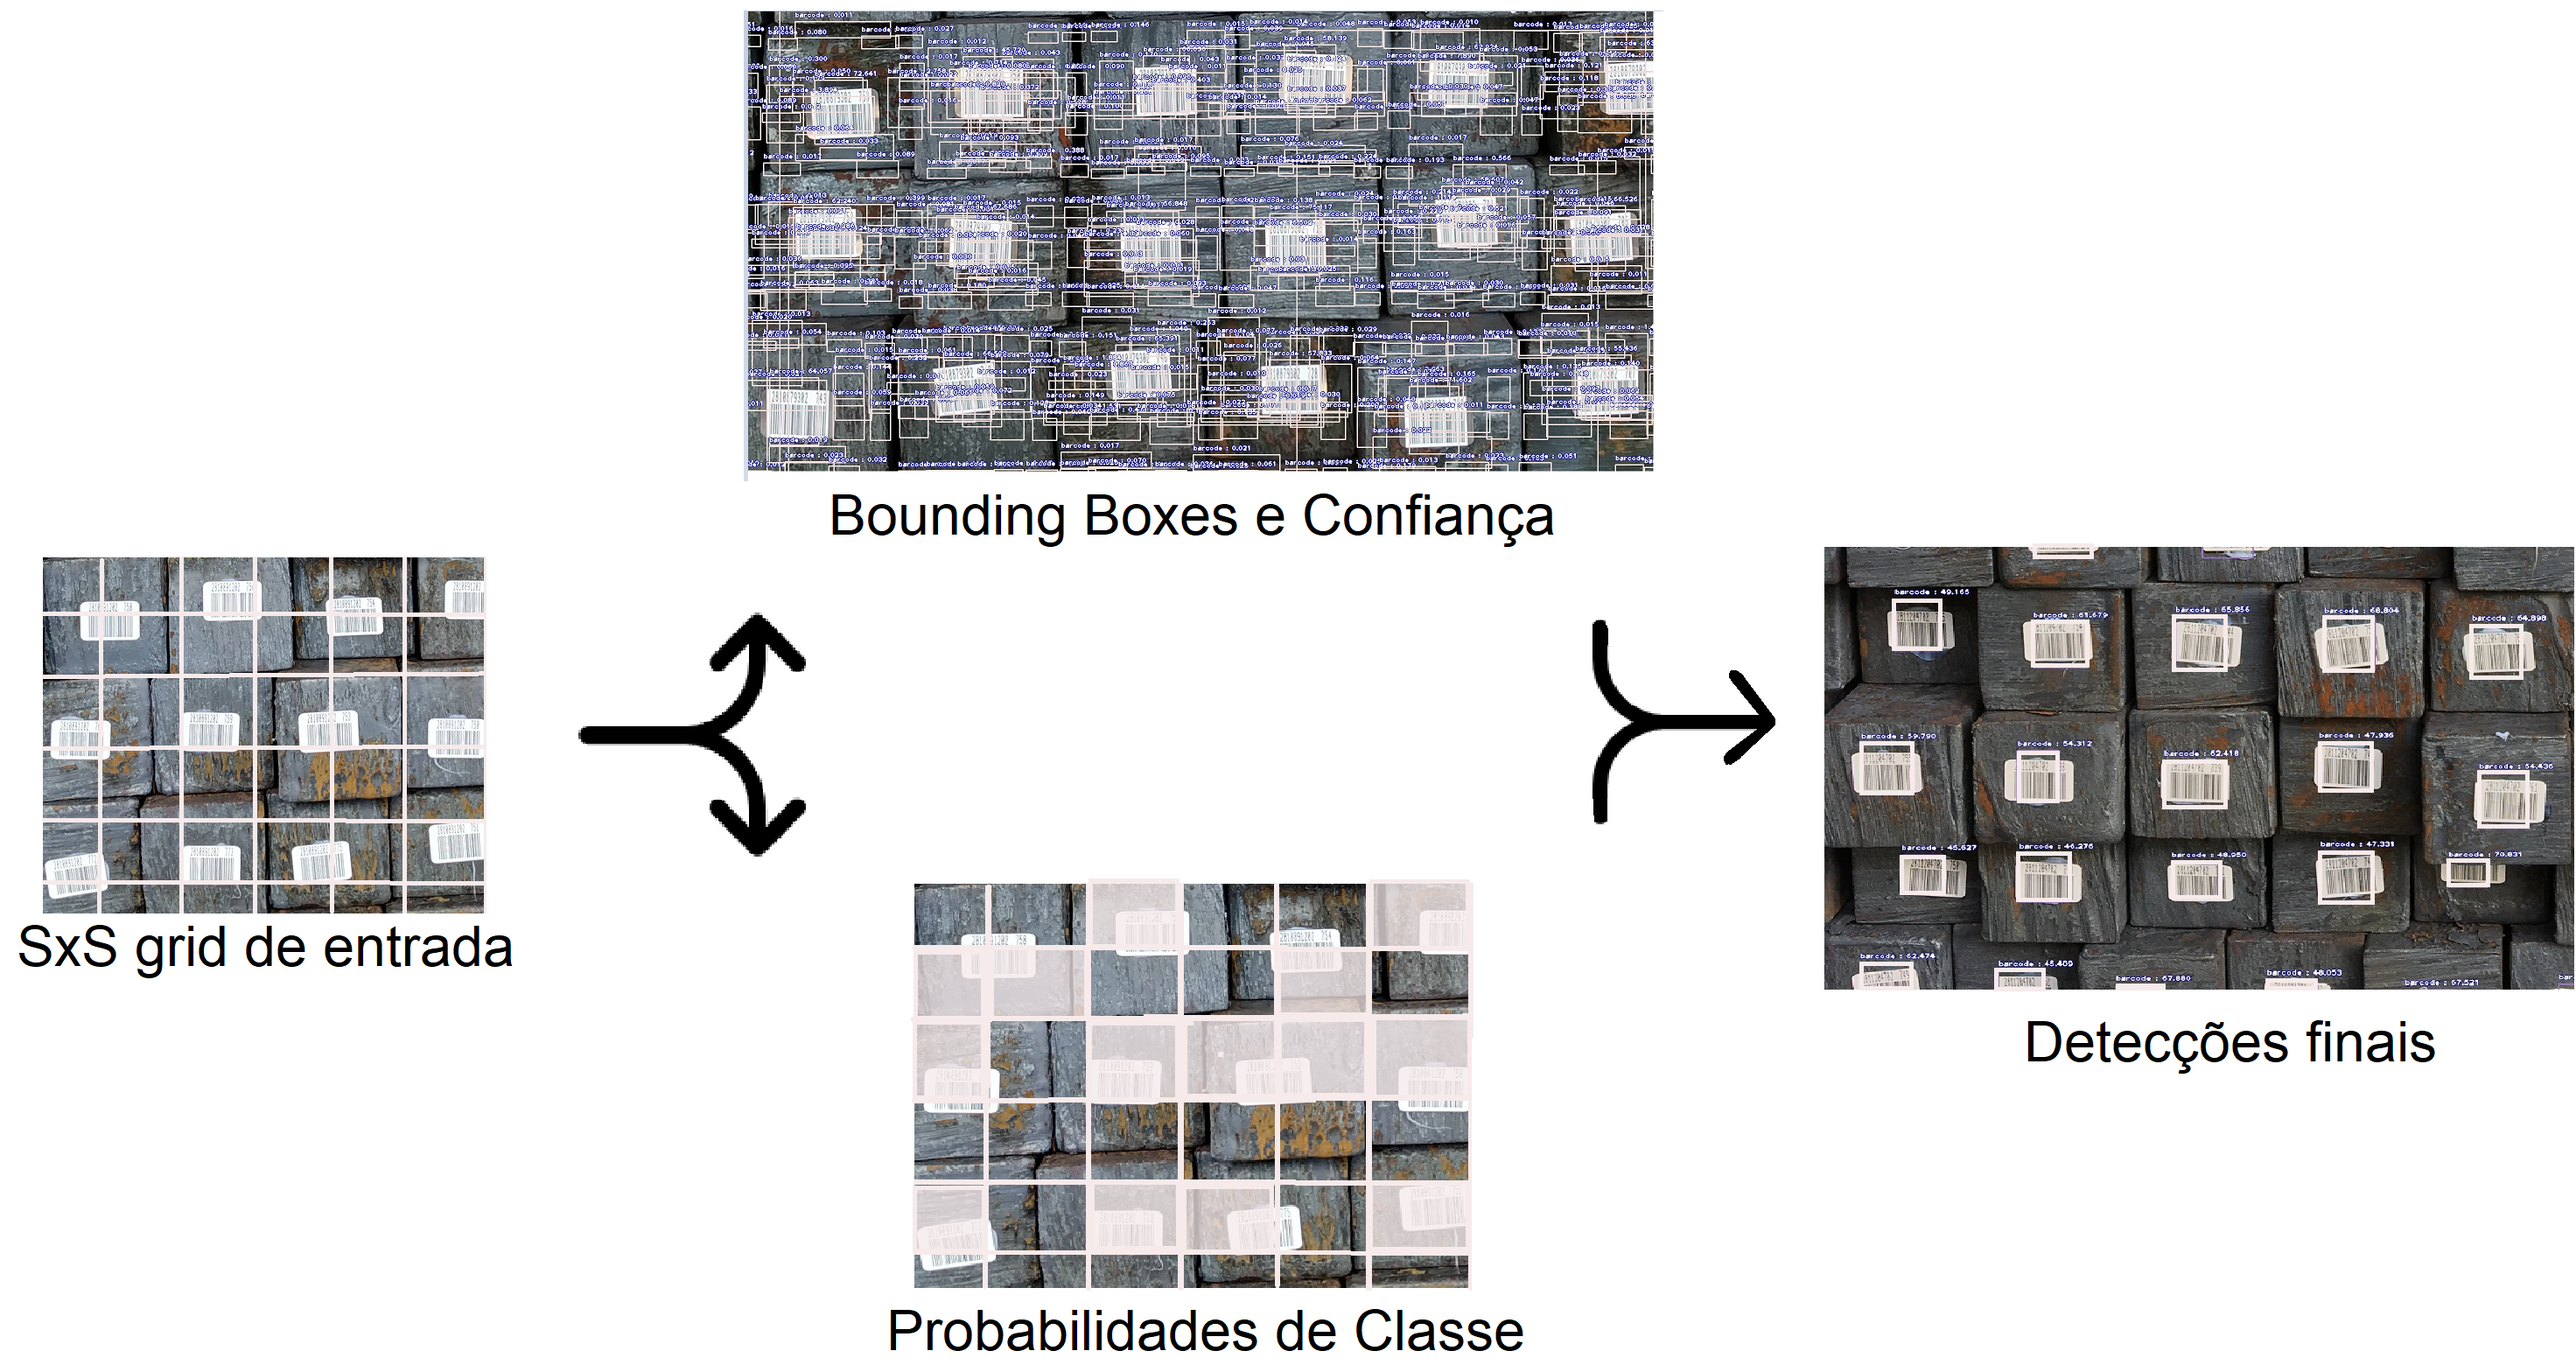
\includegraphics[scale=0.2]{figuras/MachineLearning/yolo.png}
		\caption{YOLO}
		\label{fig:yolo}
\end{figure}

No modelo de detecção YOLO (Figura \ref{fig:yolo}) uma única rede convolucional prediz tanto os \textit{bounding boxes} quanto as probabilidades de pertinencia a classe de cada objeto detectado. Para isso, YOLO funciona da seguinte forma:

\begin{itemize}
    \item Toma-se uma imagem e divide-se-a em um grid SxS de células (S = 6);
    \item Usando o \textit{grid} como referência, gera-se N \textit{bounding boxes};
    \item \textit{Bounding boxes} com probabilidade acima de um limiar são selecionados e usados para localizar o objeto dentro da imagem.
\end{itemize}

Cada célula do  \textit{grid} é usada para predizer B  \textit{bbox} e C probabilidades de classe. O conceito de interseção sobre união (IoU) tem um papel importante e a confiança de uma predição em YOLO é dada por:

\begin{equation}
    Confianca = p_r(Object) X IoU_{pred}^{truth} , p_r(Object) \in \left \{ 1\right.,\left.0\right \}
\end{equation}

Em que, quando o \textit{target} estiver na \textit{grid}, \(p_r(Object)\) = 1 e 0 caso contrário. \(IoU_{pred}^{truth}\) é usado para denotar a interseção sobre união e a previsão da \textit{bbox}. A confiança reflete se a \textit{grid} contém objetos e a precisão da \textit{bbox} prevista. Quando várias \textit{bbox} detectam o mesmo \textit{target}, o YOLO usa o método de não supressão máxima (NMS) para selecionar a melhor \textit{bbox}.

%------------------------------------------------

\section{Aplicação Web} \label{sec:web}

Neste seção mostraremos as etapas necessárias de criação da aplicação web desenvolvida para consumir os resultados do sistema de \textit{Deep Learning} mostrado anteriormente. 

O sistema web foi criado para facilitar o gerenciamento, visualização e rastreabilidade das corridas para o operador através de um \textit{layout} amigável.

Para essa etapa, utilizaremos a linguagem Node.JS para implementar o \textit{back-end} e as linguagens HTML, CSS, EJS\footnote{O EJS é uma engine de visualização, com ele conseguimos de uma maneira fácil e simples transportar dados do back-end para o front-end, basicamente conseguimos utilizar códigos em javascript no html de nossas páginas.} e JavaScript para implementar o \textit{front-end}. A escolha do Node.JS foi devido aos seguintes fatores:

\begin{itemize}
    \item Instalação ser simples pois não necessita de dependência para configuração
    \item Você consegue executar aplicações Node em qualquer plataforma.
    \item I/O não bloqueante. Isso significa que quando você precisa acessar um arquivo no disco, se comunicar com um \textit{Web Service} ou acessar um banco de dados esse acesso é feito de forma assíncrona por padrão.
    \item Por ser escrito em JavaScript, pouparia grande parte dos esforço caso opte por utilizar tecnologias \textit{front-end}, que na maioria, também são escritas em JavaScript.
\end{itemize}
 
%------------------------------------------------

\subsection{Node.JS}

O Node.JS, também conhecido como Node, é uma estrutura EDA\footnote{Maneira de realizarmos a comunicação entre sistemas que consiste, principalmente em operações assíncronas além de permitir aplicativos escalonáveis e gerar menos acoplamento entre os serviços, permitindo uma arquitetura fortemente flexível.} de código aberto para o desenvolvimento de aplicativos JavaScript em servidores. É baseado no \textit{runtime} do Google, chamado de motor V8. O V8 e o Node são implementados em C e C++, focados no desempenho e baixo consumo de memória. Embora o V8 suporte principalmente o uso de JavaScript no navegador, o Node foca no suporte de processos de servidores \cite{Tilkov2010}.

O Node é um dos \textit{frameworks} mais famosos que suportam o desenvolvimento de servidores utilizando o JavaScript \cite{Tilkov2010}.

%------------------------------------------------

\subsection{HTML}

Para publicar informações para distribuição global, é preciso uma linguagem universalmente compreendida. A linguagem de publicação usada pela WWW\footnote{WWW é um sistema de documentos dispostos na Internet que permitem o acesso às informações apresentadas no formato de hipertexto.} é HTML (da HyperText Markup Language).\citeauthor{html}

O HTML fornece aos autores os meios para: 
\begin{itemize}
    \item Publicar documentos on-line com títulos, texto, tabelas, listas, fotos, etc. 
    \item Recuperar informações on-line por meio de links de hipertexto, com o clique de um botão. 
    \item Criar formulários para realizar transações com serviços remotos, para uso em busca de informações, reservas, pedidos de produtos, etc. 
    \item Incluir planilhas, videoclipes, clipes de som e outros aplicativos diretamente em seus documentos.
\end{itemize}

%------------------------------------------------

\subsection{CSS}
De acordo com \citeauthor{css}, um dos padrões fundamentais do W3C \footnote{Trata-se de uma organização internacional responsável pelos protocolos e padronização da WWW, a rede mundial de computadores.} para o desenvolvimento de aplicativos da web é o \textit{Cascading Style Sheets}(CSS) \cite{Casca8378199:online}. CSS é uma linguagem para definir a semântica de apresentação dos elementos HTML, incluindo seu posicionamento, layout, cor e fontes. A principal mecanismo por trás da adoção do CSS tem sido a separação da estrutura da apresentação. Embora essa separação de preocupações ajude a evolução de um aplicativo da Web no que diz respeito à estrutura e ao conteúdo, o código CSS em si não é fácil de manter.\cite{badros1999constraint}

Escrever código CSS não é trivial \cite{quint2007editing}. Requer interação humano-computador, design gráfico, além de habilidades de programação na web \cite{keller2010css}. Além disso, a linguagem possui várias características, como especificidade de herança, cascata e seletor, o que torna o entendimento de como as propriedades CSS são aplicadas aos elementos DOM em tempo de execução, uma tarefa assustadora para desenvolvedores da web.

%------------------------------------------------

% \subsection{Docker}

% Docker é um projeto \textit{open source} que foi inicialmente lançado em 2013, atraiu grande atenção na industria de TI. É uma plataforma de conteinerização que possibilita usuários a construir sua aplicação dentro de um conteiner e transferir conteiners através de máquinas com diferentes sistemas operacionais de um jeito simples. \cite{chang2017kubernetes}

% Existem três componentes principais do Docker:

% \begin{itemize}
% 	\item \textit{Docker images}: são \textit{templates} de leitura que servem como base para a criação de conteiners.;
% 	\item \textit{Docker registries}: é o local onde estão uma grande coleção de \textit{Docker images}.;
% 	\item \textit{Docker containers}: são as instâncias virtuais em que as aplicações estão rodando. Cada conteiner contem uma aplicação rodando e todas os seus arquivos de dependências, como o código, bibliotecas e utilitários do sistema.
% \end{itemize}

% A construção de imagens pode ser feita de duas maneiras. É possível criar um conteiner através de uma imagem já existente (\textit{docker run}), realizar modificações e instalações dentro do conteiner, parar o container e depois salvar o estado atual do conteiner como uma nova imagem (\textit{docker commit}). Este processo é parecido com uma instalação clássica de uma máquina virtual, mas deve ser feito para cada imagem caso haja alguma atualização, já que as imagens são padronizadas. Para automatizar o processo, \textit{Dockerfiles} nos permite especificar uma imagem de base e uma sequência de comandos que serão executados quando a imagem é construída, juntamente com outras opções de especificações, como portas a serem expostas. A imagem é depois construída com o comando \textit{docker build}.\cite{DiPietro}


%------------------------------------------------
\section{Arquitetura do projeto}

Ao fazer a escolha da arquitetura do projeto, optamos utilizar a arquitetura de \textit{microservices} pois como teremos mais de um módulo de software com linguagens e características diferentes, ficaria mais fácil escalar e fazer manutenções de maneiras independentes.

\subsection{Microsserviços}
Seguindo a definição de \citeauthor{ms1} (\citeyear{ms1}), a arquitetura de microsserviços trata do desenvolvimento de uma aplicação que baseia na existência de diversos pequenos serviços independentes. Cada um dos serviços deve rodar em seu próprio processo independente. Estes serviços podem comunicar entre si utilizando mecanismos leves de comunicação (geralmente em torno no HTTP). Os serviços devem ser absolutamente independentes.

Um exemplo da arquitetura de microsserviços está na Figura \ref{fig:arquitetura-microsservicos}.

\begin{figure}[htbp]
	\centering
	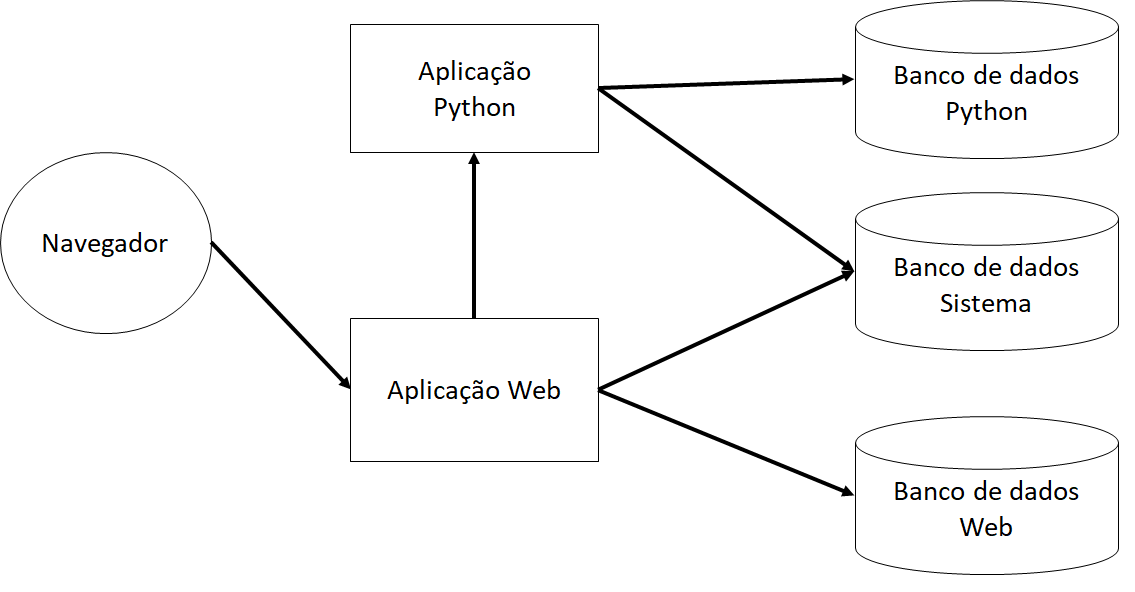
\includegraphics[width=1\linewidth]{figuras/WebService/microservices.png}
	\caption{Exemplo arquitetura de microsserviços.}
	\label{fig:arquitetura-microsservicos}
\end{figure}

Microsserviços são os resultados da decomposição funcional de uma aplicação. São caracterizados pela definição de sua interface e função no sistema. Como cada serviço deve ser independente, uma alteração na sua implementação não deve afetar o funcionamento dos demais. \cite{Pahl}

%------------------------------------------------






% ----------------------------------------------------------


\chapter{Experimentos e Resultados}

Este capítulo descreve o desenvolvimento do projeto proposto. O projeto é composto por 5 tarefas de implementação:

\begin{itemize}
    \item Montar os \textit{datasets} de \textit{barcodes} e números;
    \item Treinar, avaliar e selecionar o melhor modelo de rede neural para \textit{barcodes} e números;
    \item Implementar o algoritmo de detecção dos \textit{barcodes}.
    \item Implementar o algoritmo de detecção dos números.
    \item Implementar a aplicação web
\end{itemize}

Utilizaremos a Figura \ref{fig:imagemBase} como referência para a explicação do sistema ao longo do capítulo.

\begin{figure}[h!]
	\centering
	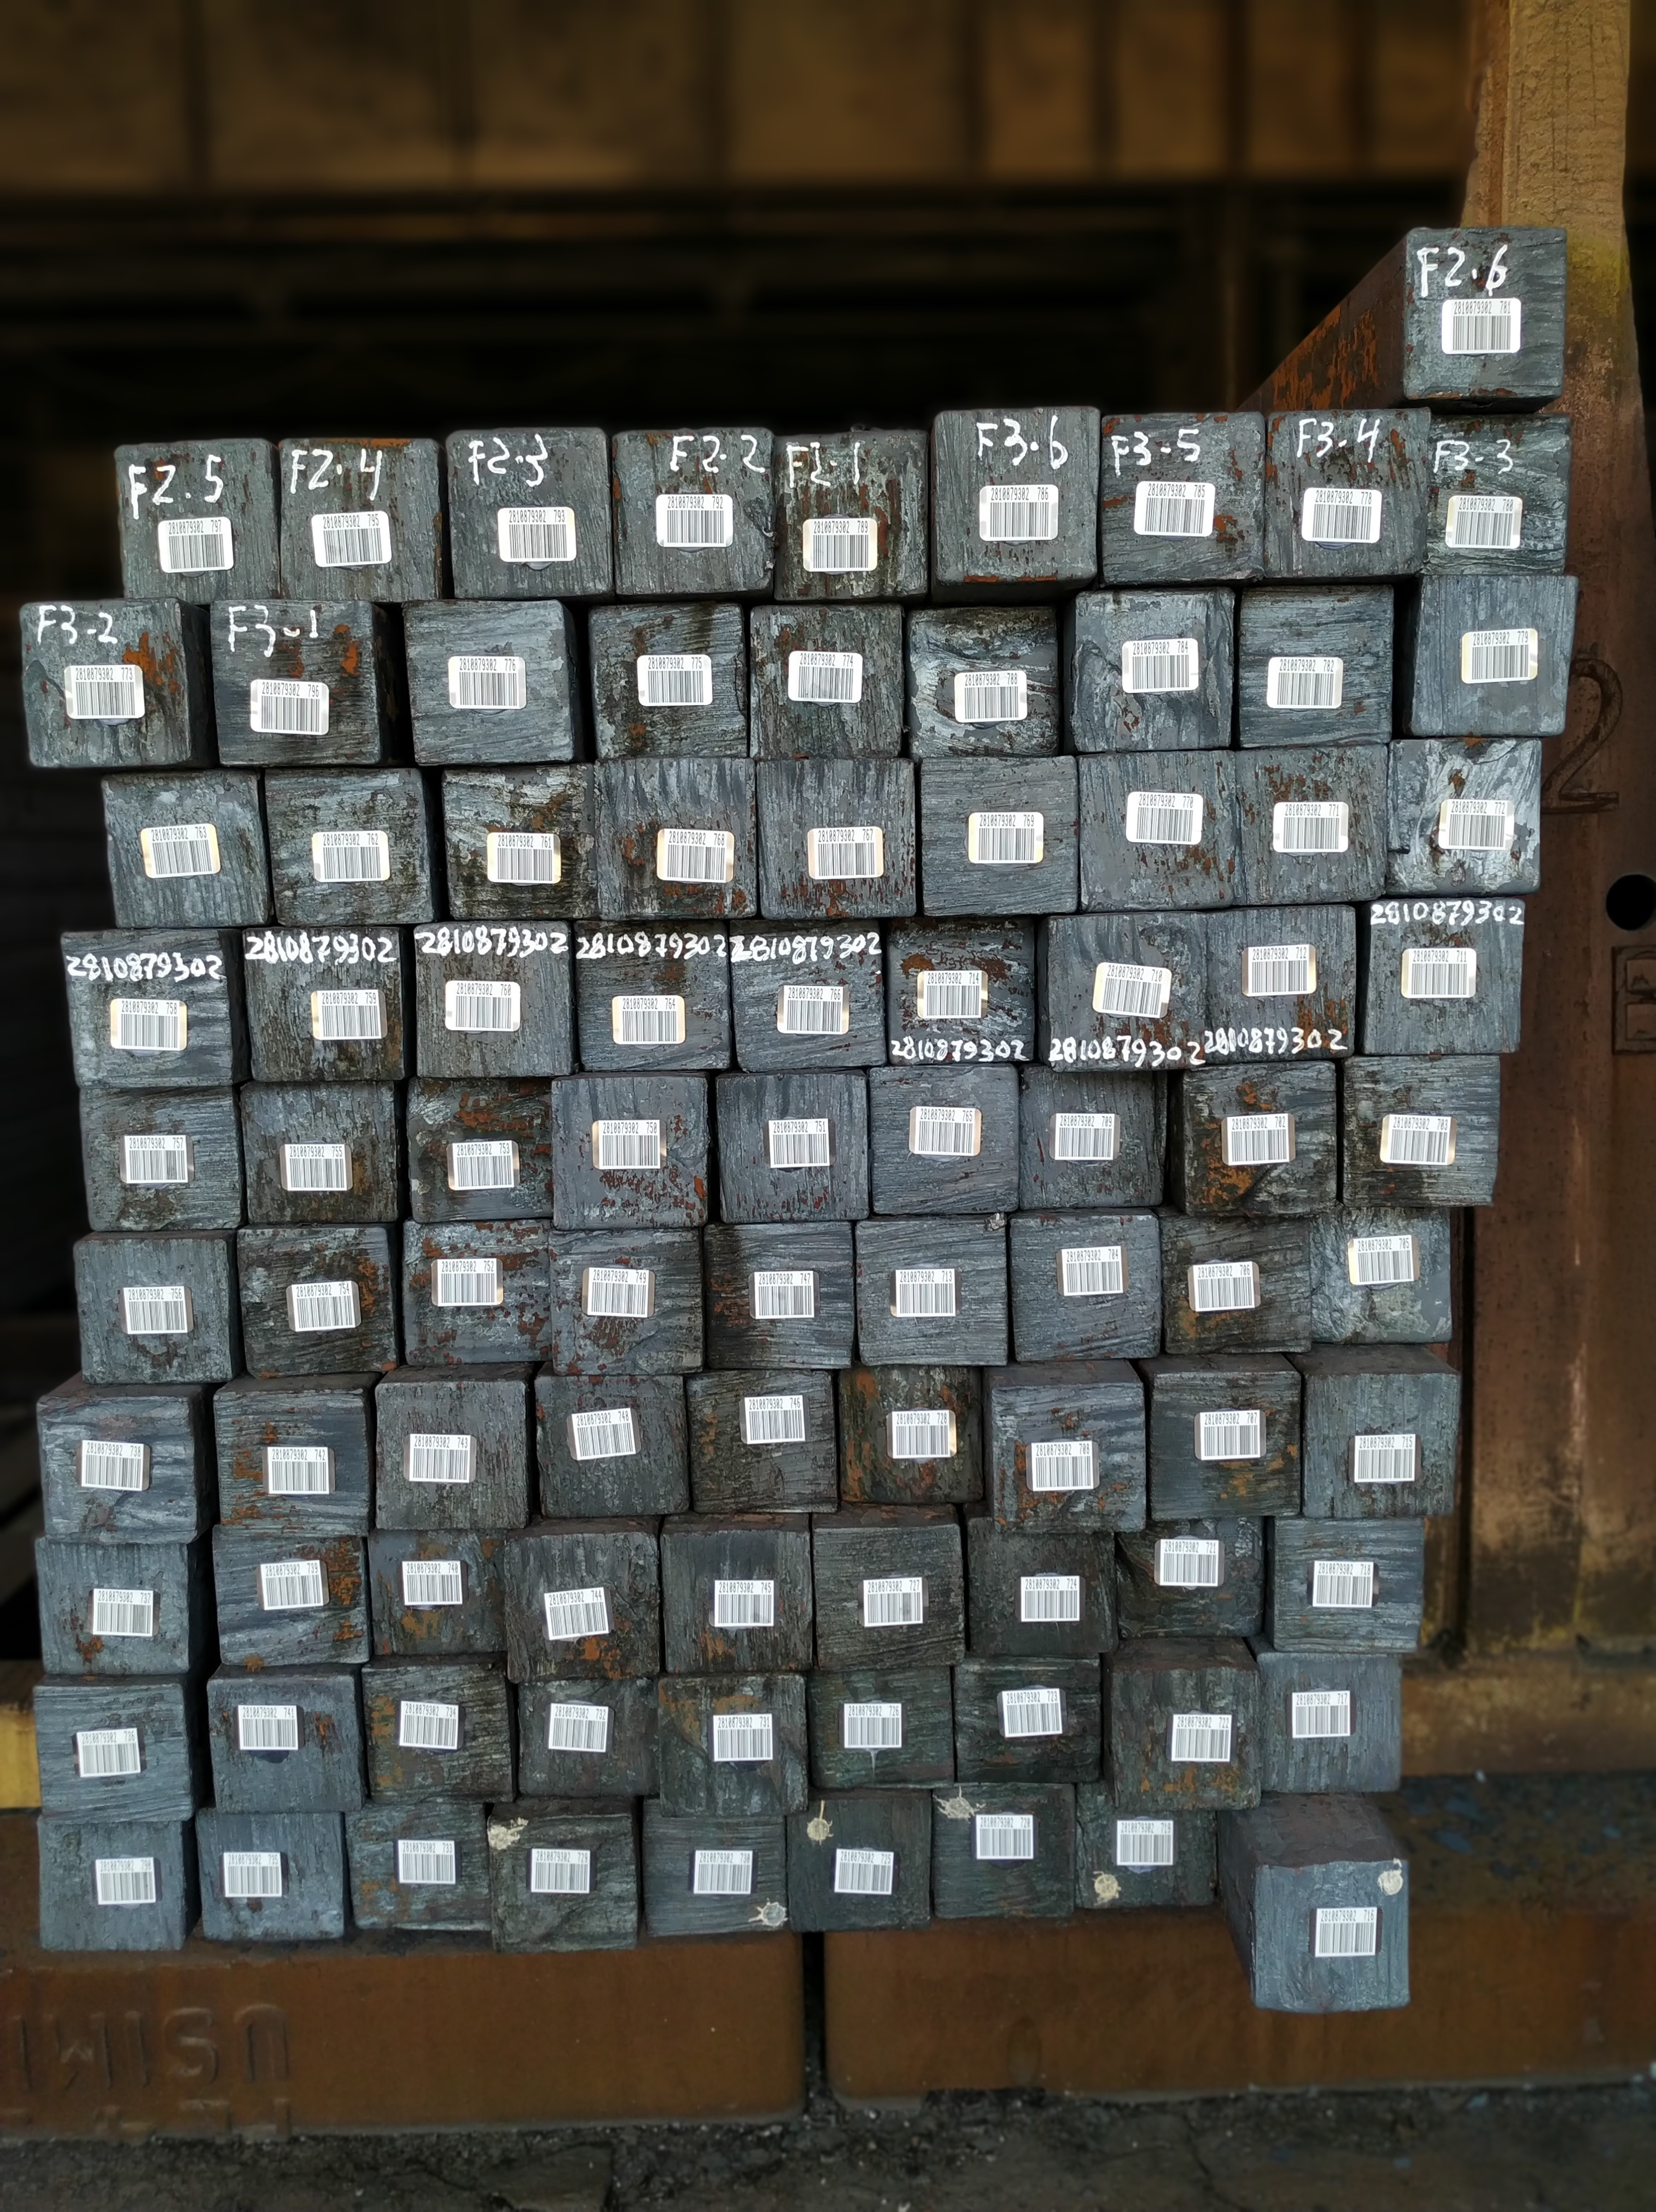
\includegraphics[width=0.5\linewidth]{figuras/img1.jpg}
	\caption{Foto tirada da corrida de tarugos.}
	\label{fig:imagemBase}
\end{figure}

\section{Montagem dos \textit{datasets}}

Nesta seção faremos a montagem dos dois \textit{datasets} para que, posteriormente, as redes neurais sejam treinadas. 

Inicialmente faremos o \textit{download} do conjunto de dados de \textit{barcodes} disponibilizado pelo laboratório \citeauthor{Arte-Lab}. Teremos por volta de 500 imagens de código de barras para o nosso \textit{dataset} inicial.

Criaremos pastas no seguinte modelo de hirarquia para nosso \textit{dataset}. (Código \ref{cod:folders})
\begin{lstlisting}[caption=Hierarquia de pastas para dataset, label=cod:folders][htb!]
        +---barcode
        |   +---train
        |   |   +---annotations
        |   |   \---images
        |   \---validation
        |       +---annotations
        |       \---images
        
        +---number
        |   +---train
        |   |   +---annotations
        |   |   \---images
        |   \---validation
        |       +---annotations
        |       \---images
\end{lstlisting}

Através do método \textit{Data Augmentation} \ref{sec:dataAugm}, aumentaremos nossa base de dados para que, após o treino, a acurácia do modelo de nossa rede neural seja a maior possível. Aplicaremos o modelo nas imagens 500 imagens resultando em $\sim~1500$ imagens de código de barras.

Utilizando a Figura \ref{fig:imagemBase}, cortaremos as etiquetas com a ajuda do software \textit{Paint} do \textit{Windows}, para sera gerada nossa base de dados de números. Optamos por utilizar os números localizados nas etiquetas uma vez que foram feitos diversos treinamento com fontes numéricas diferentes e, portanto, não obtivemos uma acurácia de detecção do número esperada.(Figura \ref{fig:barcodeDataset})

\begin{figure}[htbp]
	\centering
	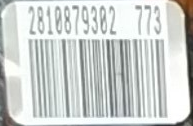
\includegraphics[width=0.25\linewidth]{figuras/MachineLearning/barcodeDataset.png}
	\caption{Montagem \textit{dataset} de números}
	\label{fig:barcodeDataset}
\end{figure}

Colocaremos 75\% das imagens na pasta validation e resto em train tanto no \textit{dataset} de \textit{barcodes} como no de números.

\subsection{Anotações das imagens}

Utilizando o software LabelImg (Subseção \ref{sub:LabelImg}), faremos as anotações das imagens para que seja gerado o arquivo PASCAL VOC no formato XML. (Figura \ref{fig:barNumAn})

\begin{figure}[htbp]
	\centering
	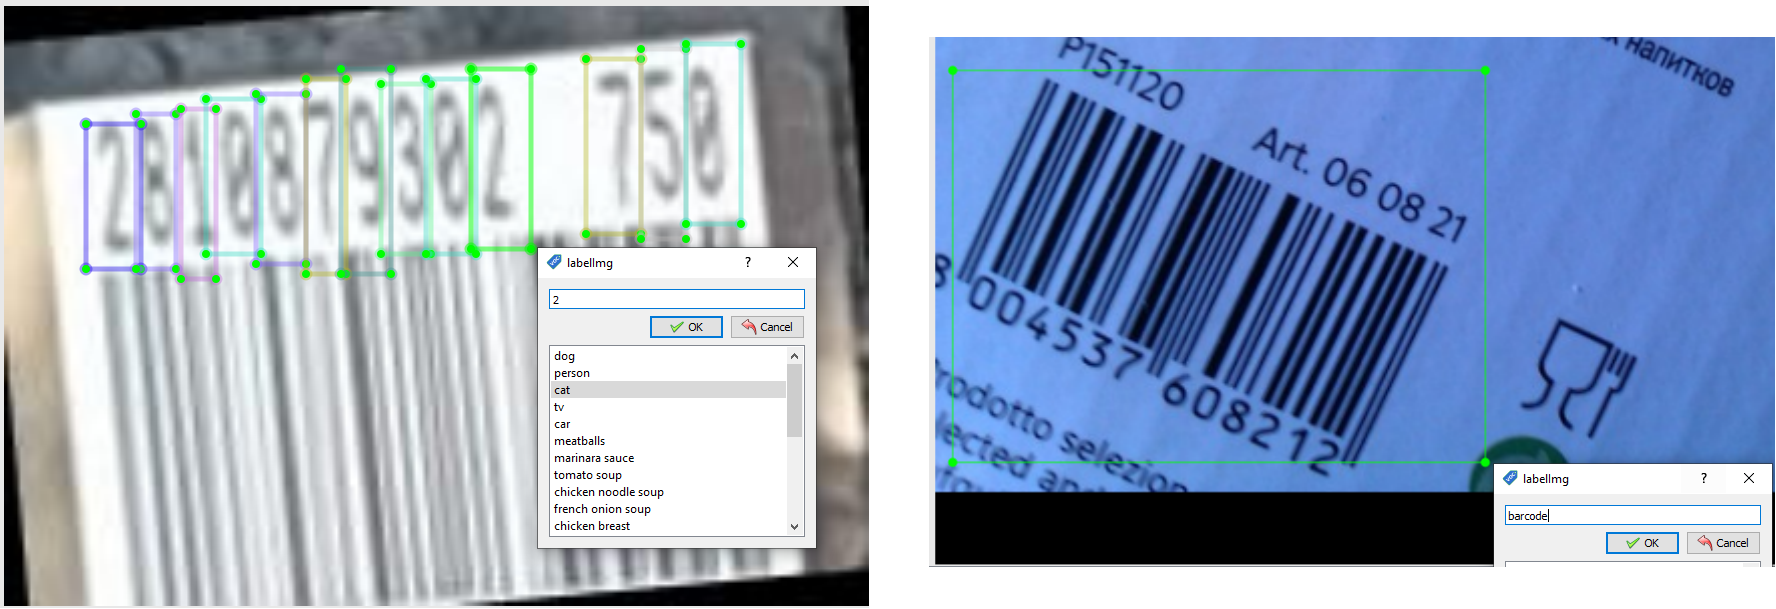
\includegraphics[width=1\linewidth]{figuras/MachineLearning/barNumAn.png}
	\caption{Anotações das imagens (Números e \textit{Barcodes})}
	\label{fig:barNumAn}
\end{figure}

\section{Fase de treinamento}

Nesta seção iremos treinar, avaliar e selecionar o melhor modelo de \textit{barcode} e número a partir da rede neural pré-treinada YOLOv3 (Subseção \ref{sub:Yolov3}).

\subsection{Treinando o modelo}

Utilizando a biblioteca ImageAI, e importando a classe \textit{DetectionModelTrainer}, treinaremos o modelo (Código \ref{cod:modeTrain}).

\begin{lstlisting}[caption=Exemplo de código do método \textit{data augmentation}, label=cod:modeTrain][htb!]
from imageai.Detection.Custom import DetectionModelTrainer

trainer = DetectionModelTrainer()
trainer.setModelTypeAsYOLOv3()
trainer.setDataDirectory(data_directory="barcode")
trainer.setTrainConfig(object_names_array=["barcode"], batch_size=4, 
                        num_experiments=11, 
                        train_from_pretrained_model=
                                            "pretrained-yolov3.h5")
trainer.trainModel()
\end{lstlisting}

\begin{itemize}
    \item \textit{object\_names\_array}: matriz que contém os nomes dos objetos em nosso \textit{dataset};
    \item \textit{batch\_size}: indica o tamanho do \textit{batch} para o treinamento;
    \item \textit{num\_experiments}: indica o número de vezes que a rede treinará sobre todas as imagens de treinamento, também chamadas de \textit{Epochs};
\end{itemize}

\begin{figure}[htbp]
	\centering
	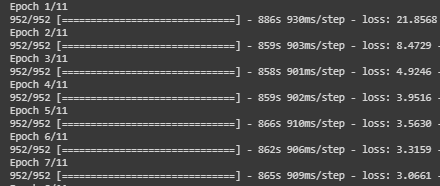
\includegraphics[width=1\linewidth]{figuras/MachineLearning/barcodeTraining.png}
	\caption{Anotações das imagens (Números e \textit{Barcodes})}
	\label{fig:barTrain}
\end{figure}

    A figura acima significa o progresso do treinamento.
\begin{itemize}
    \item Para cada experimento (\textit{Epoch}), a perda total geral de validação (por exemplo - \textit{loss}: 4.7582) é relatada.
    \item Para cada queda em \textit{loss} após uma experiência, um modelo é salvo na pasta barcode/models. Quanto menor a perda, melhor o modelo, de um modo geral, é desenhada para mostrar o quão longe estamos da solução "ideal". 
\end{itemize}

O método \textit{trainer.evaluateModel} mostrará as métricas de saída de cada modelo e a partir dos modelos gerados, avaliaremos o mAP \footnote{AP (precisão média) é uma métrica popular na medição da precisão de detectores de objetos;} de cada modelo de detecção salvo.  (Código \ref{cod:metrics})

\begin{lstlisting}[caption=Métricas de saída do modelo, label=cod:metrics][htb!]
metrics = trainer.evaluateModel(model_path="detection_model-ex-013--loss-0003.066.h5", json_path="detection_config_barcode.json", iou_threshold=0.5, object_threshold=0.3, nms_threshold=0.5)
\end{lstlisting}

Obtivemos o seguintes resultados para nossos modelos de barcodes e números:

\begin{table}[H]
	\centering
	\begin{tabular}{|l|l|l|}
		\hline
		\rowcolor[HTML]{ECF4FF} 
		\multicolumn{1}{|c|}{\cellcolor[HTML]{ECF4FF}\textit{Característica}} &
		\multicolumn{1}{|c|}{\cellcolor[HTML]{ECF4FF}\textit{Barcode}} & \multicolumn{1}{c|}{\cellcolor[HTML]{ECF4FF}\textit{Number}}\\ \hline
		\textit{Epochs} & 7 & 53\\ \hline
		\textit{Loss} & 3.066 & 12.296\\ \hline
		\textit{mAP} & 91.07\% & 77.90\%  \\ \hline
	\end{tabular}
	\caption{Melhores resultados encontrados nos modelos.}
	\label{tab:Result}
\end{table}

Ao detalhar a média de precisão dos números, podemos observar a porcentagem da probabilidade de cada número.

\begin{table}[H]
	\centering
	\begin{tabular}{|l|l|l|}
		\hline
		\rowcolor[HTML]{ECF4FF} 
		\multicolumn{1}{|c|}{\cellcolor[HTML]{ECF4FF}\textit{\textit{Number}}} &
		\multicolumn{1}{|c|}{\cellcolor[HTML]{ECF4FF}\textit{Média}}\\ \hline 
		0&  78.38\% \\ \hline
		1&  49.64\% \\ \hline
		2&  85.21\% \\ \hline
		3&  78.55\%\\ \hline
		4&  83.47\% \\ \hline
		5&  67.46\% \\ \hline
		6&  80.00\% \\ \hline
		7&  85.66\% \\ \hline
		8&  84.31\% \\ \hline
		9&  86.36\% \\ \hline
		mAP&  77.90\% \\ \hline 
		
	\end{tabular}
	\caption{Médias de precisões dos números.}
	\label{tab:avgNumbersResult}
\end{table}


\section{Implementação dos algoritmos de detecção}

Nesta seção iremos implementar os algoritmos de detecção de \textit{barcodes} e números utilizando os modelos de redes reunais treinadas na seção anterior.

\subsection{Detecção de \textit{barcode}}

Para 

\subsection{Detecção de número}


\section{Aplicação Web}
% ----------------------------------------------------------
% PARTE
% PARTE
% ----------------------------------------------------------
%\part{Resultados}
% ----------------------------------------------------------
% ---
% primeiro capitulo de Resultados
\chapter{Resultados}

% Neste Capítulo encontram-se os experimentos realizados com os sistemas devidamente implementados e configurados. Discutiremos os resultados obtidos, testando os sistemas com todas as suas funcionalidades.


% \section{Configuração do Docker}

% Toda a configuração do Docker é realizada a partir do arquivo \textit{Dockerfile}, que deve ser criado no diretório do projeto em que se deseja configurar.

% No \textit{Dockerfile} alguns parâmetros devem ser passados para conseguir o resultado esperado, um deles é definir qual imagem do Docker será usada como base, no caso dos projetos desenvolvidos, todos utilizam o Node como imagem base, esta imagem é definida com o comando \textit{FROM node}.

% Outro parâmetro que precisa ser configurado é o \textit{WORKDIR}, que define o diretório que será usado como base dentro da imagem do Docker, no caso, dentro da imagem do Node.

% Um comando importante é o \textit{COPY}, que serve para copiar os arquivos do diretório raiz do Docker, para o \textit{WORKDIR} dentro da imagem do Node.

% Após copiar os arquivos, é necessário executar os comandos para instalar os pacotes dos projetos, com o comando \textit{RUN npm install}.

% Finalmente, deve-se definir um comando de entrada, que irá executar o projeto dentro da imagem no Docker, que é o comando \textit{CMD npm start}. Caso o projeto utilize alguma porta para configuração, deve-se também expor a porta para garantir o funcionamento com o comando \textit {EXPOSE numeroDaPorta}.

% O exemplo do \textit{Dockerfile} do Sistema de Usuários pode ser verificado na Figura \ref{fig:dockerfile}.

% \begin{figure}[htbp]
% 	\centering
% 	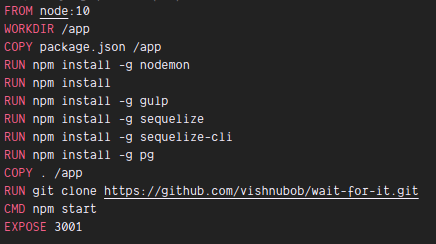
\includegraphics[width=0.7\linewidth]{figuras/dockerfile.png}
% 	\caption{Exemplo de \textit{Dockerfile} do Sistema de Usuários}
% 	\label{fig:dockerfile}
% \end{figure}

% %------------------------------------------------

% \subsection{Docker-compose}

% O \textit{Dockerfile} permite a execução única do projeto em que ele está presente, para iniciar os projetos utilizando apenas o \textit{Dockerfile} é necessário iniciar um por um.

% Para contornar este problema, o \textit{docker-compose} permite a execução de todos os projetos com apenas um comando, desde que um arquivo \textit{docker-compose.yml} esteja devidamente configurado. Este arquivo permite também a instalação e configuração automática de todos os programas utilizados neste trabalho, como o PostgreSQL, o InfluxDB, o Grafana e o Mosquitto.

% A configuração do \textit{docker-compose.yml} é simples como a do \textit{Dockerfile}, nele, deve-se especificar a versão que deseja utilizar, neste projeto foi utilizada a 3.5, com o comando \textit{version}:"3.5".

% Após a definição da versão, deve-se especificar os \textit{services}, que são as imagens que devem iniciar com o Docker. Neste projeto foram utilizados os \textit{builds} dos projetos já implementados com os devidos \textit{Dockerfiles} configurados. 

% Além dos projetos já implementados, foram especificados também os programas que foram utilizados no sistema, com o comando \textit{image:}postgres, \textit{image:}homeassistant, \textit{image:}eclipse-mosquitto, \textit{image:}grafana, \textit{image:}influxdb.

% O código implementado do \textit{docker-compose.yml} do projeto pode ser verificado no Apêndice C.



% \section{Manipulação de usuários}

% O microsserviço de usuários utiliza a porta 3001. Para utiliza-lo e testá-lo, devemos utilizar esta porta juntamente com os \textit{endpoints} disponíveis (Seção \ref{sec:usuarios}). Aqui realizaremos as consultas em todos estes \textit{endpoints} e discutiremos os resultados obtidos.

% Para criar um usuário devemos consumir\footnote{O termo "consumir um \textit{endpoint}"\  significa enviar informações para o \textit{endpoint}, esperando algum retorno, de sucesso ou falha.} o \textit{endpoint} http://localhost:3001/usuario/cadastrar passando os parâmetros via \textit{POST} no formato \textit{JSON}\footnote{Javascript Object Notation (JSON), é um formato compacto de troca de dados simples e rápida entre sistema}, como na Figura \ref{fig:cadastro}.

% A resposta deste \textit{endpoint} pode ser conferida na Figura \ref{fig:cadastro} e, para garantir que o usuário foi incluído no banco de dados, podemos observar a Figura \ref{fig:cadastro}.

% \begin{figure}[htbp]
% 	\centering
% 	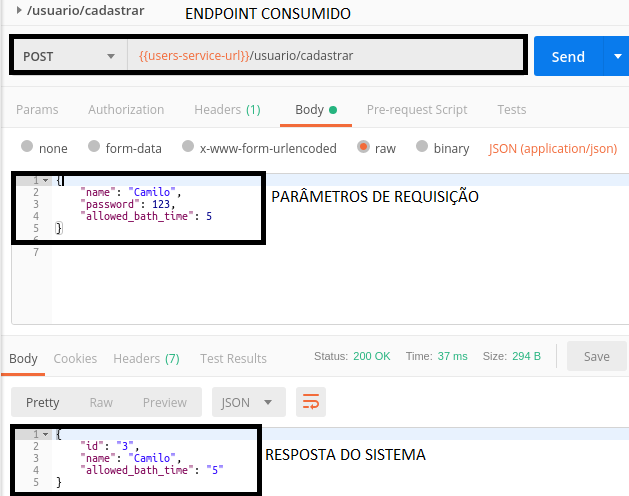
\includegraphics[width=0.7\linewidth]{figuras/postman/cadastro.png}
% 	\caption{Cadastro de usuários.}
% 	\label{fig:cadastro}
% \end{figure}

% \clearpage

% O \textit{endpoint} http://localhost:3001/usuario/editar-tempo deve ser consumido para editar o tempo máximo de banho de um usuário (Figura \ref{fig:tempo}). Para editar a senha do usuário, deve-se consumir o \textit{endpoint} http://localhost:3001/usuario/editar-senha (Figura \ref{fig:senha}).

% \begin{figure}[htbp]
% 	\centering
% 	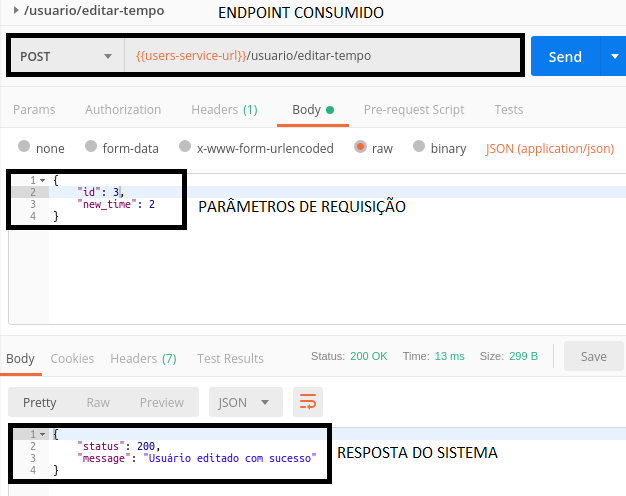
\includegraphics[width=0.7\linewidth]{figuras/postman/time.png}
% 	\caption{Edição de tempo permitido do usuário.}
% 	\label{fig:tempo}
% \end{figure}

% \begin{figure}[htbp]
% 	\centering
% 	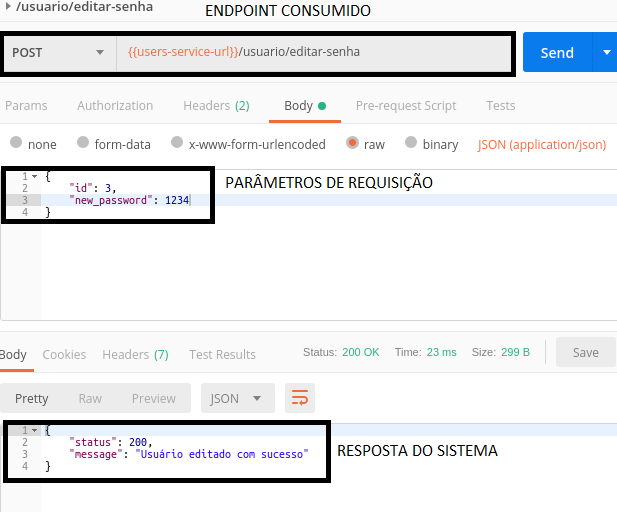
\includegraphics[width=0.7\linewidth]{figuras/postman/password.png}
% 	\caption{Edição de senha do usuário.}
% 	\label{fig:senha}
% \end{figure}

% Conseguimos cadastrar um banho ao consumir o \textit{endpoint} http://localhost:3001/banho via \textit{POST} com os parâmetros e resposta mostrados na Figura \ref{fig:banho}.

% \begin{figure}[htbp]
% 	\centering
% 	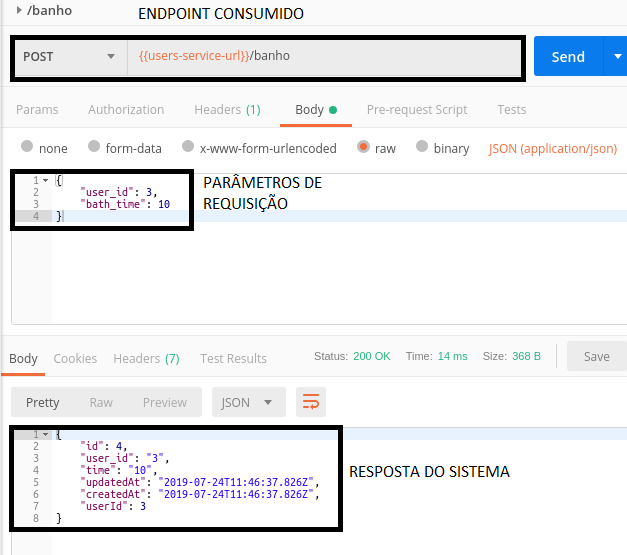
\includegraphics[width=0.7\linewidth]{figuras/postman/bathsinclude.png}
% 	\caption{Adicionando banhos ao usuário.}
% 	\label{fig:banho}
% \end{figure}

% Para recuperar as informações de um usuário, basta consumir o \textit{endpoint} \break http://localhost:3001/usuario/idDoUsuario, com o método \textit{GET}, obtendo o resultado da Figura \ref{fig:usuario}.

% \begin{figure}[htbp]
% 	\centering
% 	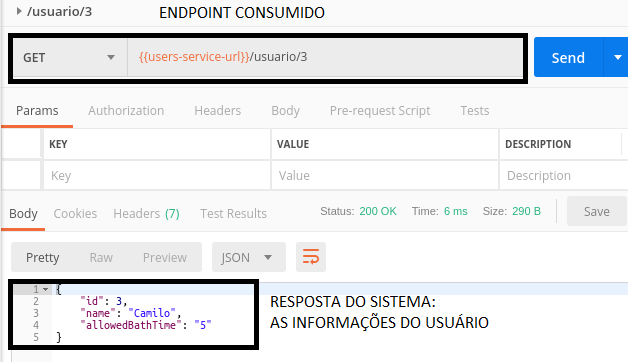
\includegraphics[width=0.7\linewidth]{figuras/postman/getuser.png}
% 	\caption{Recuperar dados do usuário.}
% 	\label{fig:usuario}
% \end{figure}

% Conseguimos as informações de todos os banhos dos usuários consumindo o \textit{endpoint} http://localhost:3001/banho/idDoUsuario, via \textit{GET}, e conseguiremos o resultado exibido na Figura \ref{fig:banhos}.

% \begin{figure}[htbp]
% 	\centering
% 	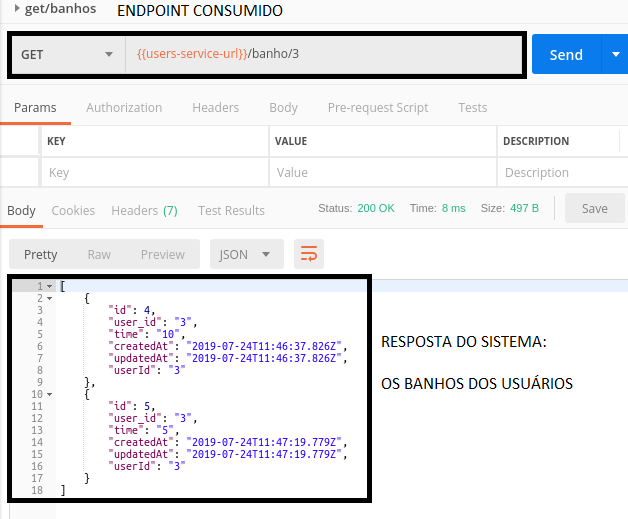
\includegraphics[width=0.7\linewidth]{figuras/postman/getbanhos.png}
% 	\caption{Recuperar dados de banhos do usuário.}
% 	\label{fig:banhos}
% \end{figure}

% Finalmente, podemos autenticar os usuários enviando via \textit{POST} os parâmetros para o \textit{endpoint} http://localhost:3001/usuario/autorizar, obtendo como resposta a Figura \ref{fig:allowedtrue}, para usuário autenticado, e Figura \ref{fig:allowedfalse}, para usuário não autenticado, caso a senha esteja errada.

% \begin{figure}[htbp]
% 	\centering
% 	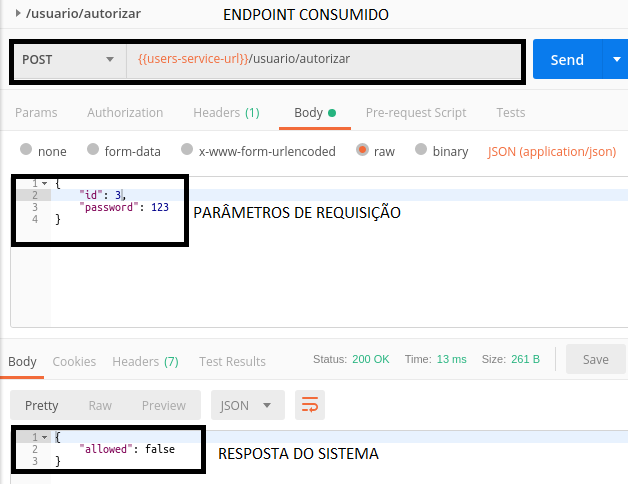
\includegraphics[width=0.7\linewidth]{figuras/postman/allowedfalse.png}
% 	\caption{Exemplo de usuário não autorizado.}
% 	\label{fig:allowedfalse}
% \end{figure}

% \begin{figure}[htbp]
% 	\centering
% 	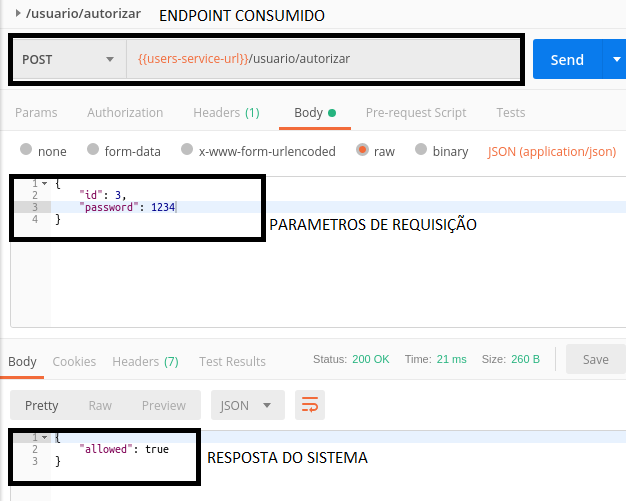
\includegraphics[width=0.7\linewidth]{figuras/postman/allowedtrue.png}
% 	\caption{Exemplo de usuário autorizado.}
% 	\label{fig:allowedtrue}
% \end{figure}

% \section{Visualização via Grafana}

% Os dados para a visualização no Grafana foram gerados pelo Sistema de simulação de dados (Seção \ref{sec:sistemasimulacao}).

% Ao autenticar um usuário, um sinal é enviado ao tópico do atuador (Seção \ref{sec:valvula}) e o sinal emulado do sensor YF-S201 (Seção \ref{sec:sensor}) inicia a simulação do fluxo, que é automaticamente enviado para o InfluxDB via Sistema de comunicação MQTT (Seção \ref{sec:sistemacomunicacao}), podendo ser visualizado no Grafana. Os gráficos do grafana podem ser acessados via http://localhost:3003, como na Figura \ref{fig:grafanahome}.

% Pode ser observado na Figura \ref{fig:grafana-graph} um gráfico do fluxo simulado pelo sensor no horário de 16h40m até 17h00m. Existem dois gráficos com cores diferentes, cada cor é referente a um usuário.

% \begin{figure}[htbp]
% 	\centering
% 	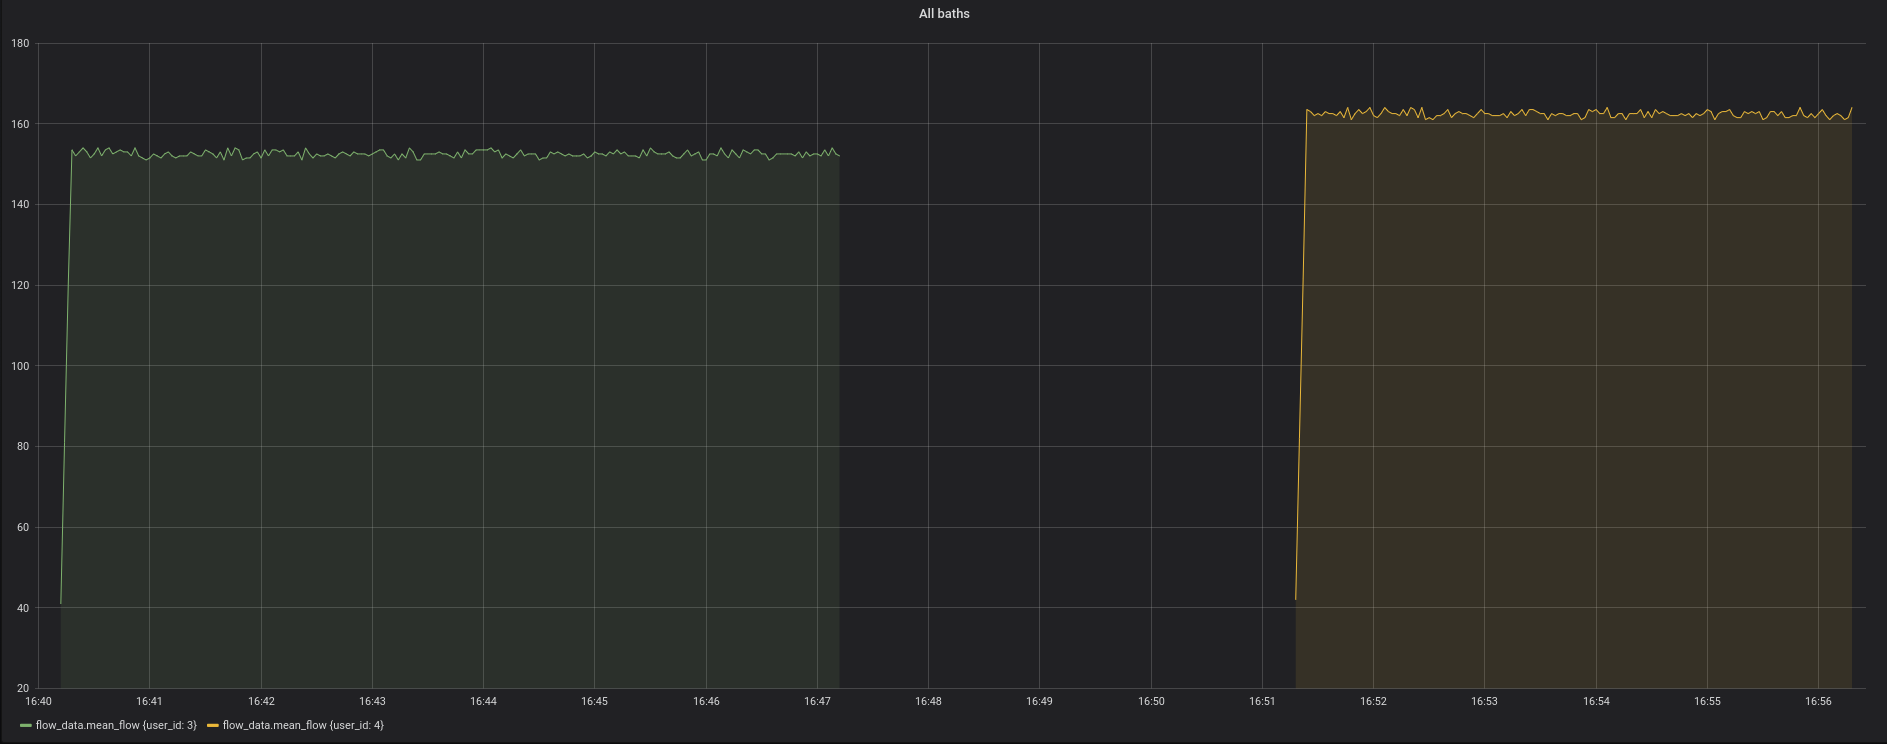
\includegraphics[width=1\linewidth]{figuras/grafanagraph.png}
% 	\caption{Exemplo do gráfico no Grafana para usuários diferentes.}
% 	\label{fig:grafana-graph}
% \end{figure}

% \section{Estado do atuador via HomeAssistant}

% O HomeAssistant é acessado via http://localhost:8123. Ao acessar o link, observamos os estado dos sensores dos usuários cadastrado na Figura \ref{fig:homeassistant-off}, que encontram-se em estado desligado. Ao digitar corretamente a senha, o estado do sensor muda para ligado, como observado na Figura \ref{fig:homeassistant-on}.

% \begin{figure}[htbp]
% 	\centering
% 	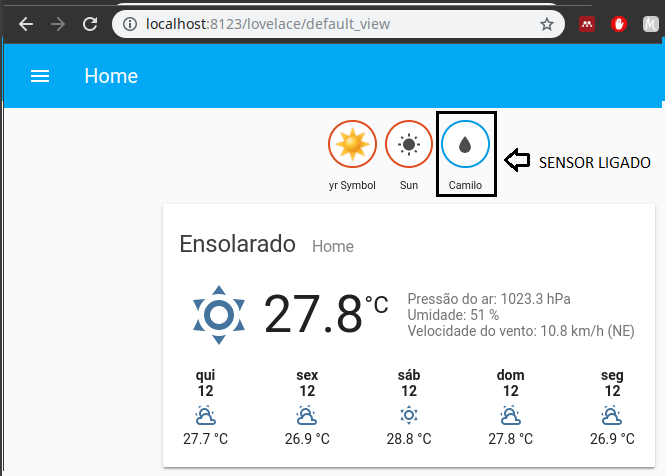
\includegraphics[width=0.6\linewidth]{figuras/homeassistanton.png}
% 	\caption{Exemplo do sensor no HomeAssistant quando ligado.}
% 	\label{fig:homeassistant-on}
% \end{figure}

% \begin{figure}[htbp]
% 	\centering
% 	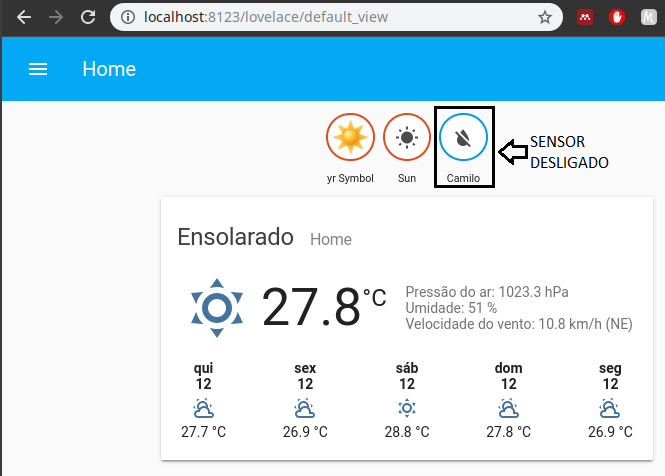
\includegraphics[width=0.6\linewidth]{figuras/homeassistantoff.png}
% 	\caption{Exemplo do sensor no HomeAssistant quando desligado.}
% 	\label{fig:homeassistant-off}
% \end{figure}

% Ao cadastrar um usuário, o seu sensor é inserido no HomeAssistant automaticamente (Figura \ref{fig:homeassistant-new}).

% \begin{figure}[htbp]
% 	\centering
% 	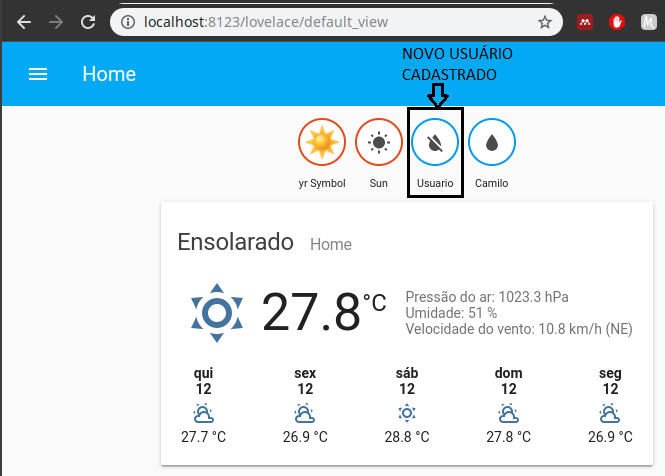
\includegraphics[width=1\linewidth]{figuras/homeassistantnewuser.png}
% 	\caption{Exemplo de um novo sensor quando um novo usuário é cadastrado.}
% 	\label{fig:homeassistant-new}
% \end{figure}



% ----------------------------------------------------------
% Finaliza a parte no bookmark do PDF
% para que se inicie o bookmark na raiz
% e adiciona espaço de parte no Sumário
% ----------------------------------------------------------
%\phantompart
% ---
% Insere arquivo de Considerações Finais ou Conclusões
% ---
\chapter{Considerações Finais}

 Este trabalho propõe um sistema capaz detectar código de barras e números através de uma imagem. Os sistemas de reconhecimento de objetos e aplicação web foram implementados. Como mostrado, a implementação é capaz identificar os códigos de barras, identificar os números e mostrá-los em uma aplicação através de telas e imagens.
 
Ao final do desenvolvimento do projeto e dos resultados apresentados, pode-se concluir que o sistema é eficaz na identificação dos objetos e na gestão do status da corrida, podendo ser um grande aliado na redução da misturas de aço, automatização do processo e na segurança do trabalhador.

Como trabalhos futuros, sugere-se a implementação física do sistema em uma unidade industrial, bem como a utilização da foto em tempo real para rodar o sistema. 

Para melhorar a assertividade ainda mais dos objetos, seria interessante testar mais opções de treinamentos para os modelos da rede neural. Para isso, são necessários testes extensivos. Os tópicos abaixo provavelmente ajudariam a aumentar a acurácia do modelo:

\begin{itemize}
    \item Aumentar o \textit{dataset} de treinamento e validação dos modelos utilizando apenas imagens originais. (Figura \ref{fig:imagemBase})
    \item Criar as \textit{bounding boxes} utilizando o LabelImg [0,1,2,3,4,5,6,7,8,9] direto nas imagens originais + imagens com \textit{data augmentation};
\end{itemize}

% ----------------------------------------------------------
% ELEMENTOS PÓS-TEXTUAIS
% ----------------------------------------------------------
\postextual
% ----------------------------------------------------------
% ----------------------------------------------------------
% Referências
% ----------------------------------------------------------
\bibliography{abntex2-modelo-references}
% ----------------------------------------------------------
% Glossário
% ----------------------------------------------------------
%
% Consulte o manual da classe abntex2 para orientações sobre o glossário.
%
%\glossary

% ----------------------------------------------------------
% Apêndices
% ----------------------------------------------------------
%(Lembre-se: Apendices são de autoria do próprio autor do texto. 
% Anexos são elementos de autorias de outros, que o autor do texto julga interessante apresentar)
% ---
% Inicia os apêndices: 
% ---
\begin{apendicesenv}

% Imprime uma página indicando o início dos apêndices
\partapendices
% ---
% Insere arquivo com os apendices A e B
\chapter{Sistema de identificação} \label{ap:ident}

Neste apêndice encontram-se algumas partes importantes dos códigos do método de \textit{Data Augmentation}, do Sistema de Identificação de Código de barras e de Identificação de Números. Os códigos inteiros podem ser encontrados através do \textit{link}:\url{https://github.com/AntonioHenriqueAC/Barcode_Number-Recognition/tree/master/google_colab}
\newline

\begin{lstlisting}[caption=Método de \textit{Data augmentation}]
import os
import random
from scipy import ndarray

# image processing library
import skimage as sk
from skimage import transform
from skimage import util
from skimage import io

def random_rotation(image_array: ndarray):
    # pick a random degree of rotation between 25% on the left and 25% on the right
    random_degree = random.uniform(-10, 10)
    return sk.transform.rotate(image_array, random_degree)

def random_noise(image_array: ndarray):
    # add random noise to the image
    return sk.util.random_noise(image_array)

def horizontal_flip(image_array: ndarray):
    # horizontal flip doesn't need skimage, it's easy as flipping the image array of pixels !
    return image_array[:, ::-1]

# dictionary of the transformations we defined earlier
available_transformations = {
    'rotate': random_rotation,
    'noise': random_noise,
    'horizontal_flip': horizontal_flip
}


from google.colab import drive
drive.mount('/content/drive')


folder_path = "PATH DAS IMAGENS ORIGINAIS"
num_files_desired = 1000

# find all files paths from the folder
images = [os.path.join(folder_path, f) for f in os.listdir(folder_path) if os.path.isfile(os.path.join(folder_path, f))]

num_generated_files = 0
while num_generated_files <= num_files_desired:
    # random image from the folder
    image_path = random.choice(images)
    # read image as an two dimensional array of pixels
    image_to_transform = sk.io.imread(image_path)
    # random num of transformation to apply
    num_transformations_to_apply = random.randint(1, len(available_transformations))

    num_transformations = 0
    transformed_image = None
    while num_transformations <= num_transformations_to_apply:
        # random transformation to apply for a single image
        key = random.choice(list(available_transformations))
        transformed_image = available_transformations[key](image_to_transform)
        num_transformations += 1

        new_file_path = '%s/augmented_image_%s.jpg' % (folder_path, num_generated_files)

        # write image to the disk
        io.imsave(new_file_path, transformed_image)
        num_generated_files += 1
\end{lstlisting}

%----------------------------------------------------------------------------
\newpage

\begin{lstlisting}[caption=Treinamento do modelo de \textit{barcodes}]
# Conectando o drive ao colab
from google.colab import drive
drive.mount('/content/drive')
        
# Baixando as bibliotecas necessarias
!pip3 install tensorflow-gpu==1.13.1
!pip3 install imageai --upgrade

# Treinar novo Modelo !
# 1. Baixando a CNN pre-treinada
!wget https://github.com/OlafenwaMoses/ImageAI/releases/download/essential-v4/pretrained-yolov3.h5

# Carregando os arquivos do drive no colab
!unzip "/content/drive/My Drive/Colab/datasets/barcode.zip"

# 3. Treinando o modelo
from imageai.Detection.Custom import DetectionModelTrainer

trainer = DetectionModelTrainer()
trainer.setModelTypeAsYOLOv3()
trainer.setDataDirectory(data_directory="barcode")
trainer.setTrainConfig(object_names_array=["barcode"], batch_size=4, num_experiments=11, train_from_pretrained_model="pretrained-yolov3.h5")
trainer.trainModel()


# 4. Avaliando os modelos gerados
metrics = trainer.evaluateModel(model_path="barcode/models", json_path="/content/drive/My Drive/Colab/json/detection_config_barcode.json", iou_threshold=0.5, object_threshold=0.3, nms_threshold=0.5)
\end{lstlisting}

%----------------------------------------------------------------------------
\newpage

\begin{lstlisting}[caption=Funções de eliminação de \textit{Bounding Boxes} sobrepostas e duplicadas, label=ap:IoU]
	# determine the (x, y)-coordinates of the intersection rectangle
	xA = max(boxA[0], boxB[0])
	yA = max(boxA[1], boxB[1])
	xB = min(boxA[2], boxB[2])
	yB = min(boxA[3], boxB[3])
	# compute the area of intersection rectangle
	interArea = max(0, xB - xA + 1) * max(0, yB - yA + 1)
	# compute the area of both the prediction
	# rectangles
	boxAArea = (boxA[2] - boxA[0] + 1) * (boxA[3] - boxA[1] + 1)
	boxBArea = (boxB[2] - boxB[0] + 1) * (boxB[3] - boxB[1] + 1)
	# compute the intersection over union by taking the intersection
	# area and dividing it by the sum of prediction
	# areas - the interesection area
	iou = interArea / float(boxAArea + boxBArea - interArea)
	# return the intersection over union value
	return iou

def boxArea(boxA, boxB):
	boxAArea = (boxA[2] - boxA[0] + 1) * (boxA[3] - boxA[1] + 1)
	boxBArea = (boxB[2] - boxB[0] + 1) * (boxB[3] - boxB[1] + 1)
	return boxAArea/boxBArea

def removeDuplicatesLoop(detections):
	i=0
	k=0
	for i, detection in enumerate(detections):
		for k, detection in enumerate(detections):
					inter = bb_intersection_over_union(detections[i]["box_points"] , detections[k]["box_points"])
					if(inter > float(0.01) and inter < float(1)):
						if(boxArea(detections[i]["box_points"] , detections[k]["box_points"]) > 1):
							detections.pop(k)
						else:
							detections.pop(i)
							removeDuplicatesLoop(detections)
							
\end{lstlisting}

%----------------------------------------------------------------------------
\newpage
\begin{lstlisting}[caption=Aumento da \textit{bouding box} e recorte dos \textit{barcodes} em imagens individuais, label=ap:AumentaBbox]

from imageai.Detection.Custom import CustomObjectDetection
from prettytable import PrettyTable

if( len(filesIMG) == len(dirs) ):
  print("Nao ha mais imagem para treinar. Por favor insira mais imagens na pasta /Imagens_Originais")
else:
  detector = CustomObjectDetection()
  detector.setModelTypeAsYOLOv3()
  detector.setModelPath(modelPath)
  detector.setJsonPath(JsonPath)
  detector.loadModel()

  detections = detector.
                    detectObjectsFromImage(input_image = InputImage, 
                    output_image_path="barcode-detected-OriginalBoxes.jpg",
                    minimum_percentage_probability=30)
                    
  for e in detections:
    e['box_points'][0] = e['box_points'][0] - 50 ## x1
    e['box_points'][1] = e['box_points'][1] - 50 ## y1
    e['box_points'][2] = e['box_points'][2] + 50 ## x2
    e['box_points'][3] = e['box_points'][3] + 50 ## y2

  removeDuplicatesLoop(detections)

  header = PrettyTable(["Nome", "Porcentagem ", "box_points"])
  for detection in detections:
    header.add_row([detection["name"], detection["percentage_probability"], detection["box_points"]])

  img = PrettyTable(["Barcodes identificados"])
  img.add_row([len(detections)])
\end{lstlisting}

%----------------------------------------------------------------------------
\newpage

\begin{lstlisting}[caption=Recorte das \textit{bounding box} e exportação para uma pasta tags-images]
matplotlib inline
import numpy as np
import skimage.io
import matplotlib.pyplot as plt
import skimage.segmentation
import cv2

if( len(filesIMG) == len(dirs) ):
  print("Nao ha mais imagem para treinar. 
  Por favor insira mais imagens na pasta '/Imagens_Originais'")
else:
  Image_with_boxes = "barcode-detected-OriginalBoxes.jpg"

  img = skimage.io.imread(InputImage)
  bbox = []

  for e in detections:
      bbox.append(e['box_points'])

  for i, (x1,y1,x2,y2) in enumerate(bbox):

      if i in {0,1,2,3,4,5,6,7,8,9}:
        i = '00' + str(i)
      
      if(int(i) > 9 and int(i) < 100):
        i = '0' + str(i)

      img2 = cv2.rectangle(img, (x1,y1), (x2,y2), (0,255,0), 0)
      out = img[y1:y2, x1:x2]

      cv2.imwrite('barcode-detected-objects/barcode-00'+str(i)+'.jpg', out)

  cv2.imwrite('barcode-detected-New.jpg', img)

  print("Boxes recortados com sucesso!")
  print("..")
  print("..")
  print("..")
  print("Imagem = 'barcode-detected-New.jpg' gerada.")
\end{lstlisting}

%----------------------------------------------------------------------------
\newpage
\begin{lstlisting}[caption=Função para fazer a diferença entre distância dos números para deletar o de menor Acurácia, label=ap:removeNumber]
def removeDuplicates():
    i=0
    for detection in detections:
      if( i != len(detections)-1 ):
          
          Xa = (detections[i]['box_points'][0] + detections[i]['box_points'][2])/2
          Ya = (detections[i]['box_points'][1] + detections[i]['box_points'][3])/2
          Xb = (detections[i+1]['box_points'][0] + detections[i+1]['box_points'][2])/2
          Yb = (detections[i+1]['box_points'][1] + detections[i+1]['box_points'][3])/2

          Dab = ( (Xb-Xa)**2 + (Yb - Ya)**2 )**1/2
          if(Dab < float(10)):
              if(detections[i]["percentage_probability"] < detections[i+1]["percentage_probability"]):
                  detections.pop(i)
              else:
                  detections.pop(i+1)
      i=i+1
\end{lstlisting}

%----------------------------------------------------------------------------

\begin{lstlisting}[caption=Identificando os números nas imagens com \textit{barcodes} individuais, label=ap:identNumber]
from imageai.Detection.Custom import CustomObjectDetection
import json
from prettytable import PrettyTable

modelPath = "Colab/models/number/detection_model-ex-034--loss-0012.508.h5"
JsonPath = "Colab/json/detection_config_number.json"

detector = CustomObjectDetection()
detector.setModelTypeAsYOLOv3()
detector.setModelPath(modelPath)
detector.setJsonPath(JsonPath)
detector.loadModel()

avgCorrida = 0

for x in range(file_count_tag):

  i=0
  soma=0
  numero=''
  execucoes = 0

  if x in {0,1,2,3,4,5,6,7,8,9}:
    x = '00' + str(x)
  
  if(int(x) > 9 and int(x) < 100):
    x = '0' + str(x)

  detections = detector.detectObjectsFromImage(input_image="Colab/Corridas/Corrida_"+str(corrida)+"/tags_images/barcode-00"+str(x)+".jpg", 
                                          output_image_path="Colab/Corridas/Corrida_"+str(corrida)+"/tags_detected/digit-detected-"+str(x)+".jpg", 
                                          display_percentage_probability=False, 
                                          minimum_percentage_probability=60)
  def boxPoints(e):
    return e['box_points']

  detections.sort(key=boxPoints)

  menor = 100
  while(len(detections) > 13):
    execucoes = execucoes + 1
    if(execucoes>10000):
      for i, detection in enumerate(detections):
        if(menor > detections[i]["percentage_probability"]):
          menor = detections[i]["percentage_probability"]   
      for k, detection in enumerate(detections):
        if(detections[k]["percentage_probability"] == menor):
          detections.pop(k)
      break
    removeDuplicates()

  img = PrettyTable(["                     Imagem                    "])
  img.add_row([x])
  header = PrettyTable(["Numero", "Porcentagem ", "box_points"])
  alert = ''
  for i in range(len(detections)):
    if(detections[i]["percentage_probability"] < 99):
      detections[i].update({"alert" : "true"})
      alert = "true"
    else:
      detections[i].update({"alert" : "false"})
      alert = "false"
    header.add_row([detections[i]["name"], detections[i]["percentage_probability"], detections[i]["box_points"]])
    soma = soma + detections[i]["percentage_probability"]
    numero = numero + ''.join(detections[i]["name"])

  if(len(detections) != 0):
    avg = soma/len(detections)
  table = PrettyTable(["Numeros", "Quantidade", "Media"])
  table.add_row([numero, len(detections), avg])
  
  avgCorrida = avgCorrida + avg
  num=numero
  config = {
      "num": num,
      "id": x,
      "acc": avg,
      "alert": alert
    }
  detections[:0] = [config]

  with open('Colab/Corridas/Corrida_'+str(corrida)+'/tags_json/tag-'+ str(x) +'.json', 'w', encoding='utf-8') as f:
    json.dump(detections, f, ensure_ascii=False, indent=4)
\end{lstlisting}


%----------------------------------------------------------------------------
\newpage

\begin{lstlisting}[caption=Criando o arquivo config-x.json]
avgCorrida = avgCorrida/float(file_count_tag)

config = {
    "numCorrida": num,
    "Status": "Inadimplente",
    "acc": avgCorrida,
    "qte": file_count_tag
}

with open('Colab/Corridas/Corrida_'+str(corrida)+'/config_'+str(corrida)+'.json', 'w', encoding='utf-8') as f:
    json.dump(config, f, ensure_ascii=False, indent=4)
\end{lstlisting}


%----------------------------------------------------------------------------
\newpage

\chapter{Aplicação Web} \label{ap:web}

Neste apêndice encontram-se algumas partes importantes dos códigos do software web desenvolvido . Os códigos inteiros podem ser encontrados através do \textit{link}: \url{https://github.com/AntonioHenriqueAC/Barcode_Number-Recognition}
\newline


%----------------------------------------------------------------------------

\begin{lstlisting}[caption=Exemplo do código dos \textit{controllers}]
var path = require('path');
var rootPath = path.join(__dirname, '../../');
var fs = require('fs');
var CorridaBs = require('../business/corrida.bs');
const image2base64 = require('image-to-base64');
const util = require('util')
var multer = require('multer');

const readDirPromise = util.promisify(fs.readdir);
const renamePromise = util.promisify(fs.rename)
const readFilePromise = util.promisify(fs.readFile)
const writeFilePromise = util.promisify(fs.writeFile)


module.exports.list = async (req, res) =>{
	var corrida = new CorridaBs();

	await callListPage();
	async function callListPage() {
		await corrida.listHome();
		const data = await corrida.list();
			res.render('list', {
			corrida: data
			})
	}

}	

module.exports.detailPage = async (req, res) => { 
	var corrida = new CorridaBs(req);

		await callDetailPage();
		async function callDetailPage() {
			let detail = await corrida.list();
			await corrida.groupCorridaDetail(req);
			let data = await corrida.listTags(req);
			
			const position = req.body.id - 1

			detail = detail[position]
			res.render('corrida-detail',{
				corrida: data,
				tags: data.length,
				detail: detail,
				position: position
			})
		}
}


module.exports.checkCorrida = async (req, res) => {
	
	let corrida = new CorridaBs();
	let targetCorrida = req.body.position;
	let dir = rootPath + 'server/corridas_config/config/';

	async function getDirectories(path) {
		const files = await readDirPromise(path);
		const file = parseInt(targetCorrida) 
		let nameFile = files[file];

		return new Promise((resolve) => {
			resolve(path + nameFile);
		})
	}
	const fileName = await getDirectories(dir)

	
	await callCheckCorrida();
	async function callCheckCorrida() {
			let resultFull = await corrida.list();

			result = resultFull[targetCorrida]
			var corridaStatus = result.status;
		
			result.Status = "Despachada"

			await writeFilePromise(fileName, JSON.stringify(result))

			if (corridaStatus == "Despachada") {
				res.render('corrida-desp');
			} else {
				res.render('corrida-check', {
				corrida: result.nuMCorrida
				})
			}
	}

}

module.exports.deleteCorrida = async (req, res) => {
var corrida = new CorridaBs();

var dir = rootPath + 'server/corridas_config/config/';
var dirDelete = rootPath + 'server/corridas_config/deleted/';


async function getDirectories(path ) {
	const files = await readDirPromise(path);
	const file = parseInt(req.body.id) - 1
	let nameFile = files[file];

	return new Promise((resolve)=>{
		resolve(path+nameFile);
	})
}

 	const result = await corrida.list()

	let targetCorrida = parseInt(req.body.id) -1;
	let corridaTarget = result[targetCorrida]

	const fileName = await getDirectories(dir)

	let moveFile = async (file, dir2) => {
		let f = path.basename(file);
		let dest = path.resolve(dir2, f);
		await renamePromise(file, dest);
	};

	await moveFile(fileName, dirDelete);

	res.render('corrida-delete', {
			corrida: corridaTarget.nuMCorrida
			})
};


module.exports.showImage = async (req, res) => {
	target = req.body.id - 1
	position = parseInt(req.body.position) + 1

	if (target >= 0 && target < 10) target = '00' + target
	if (target > 9 && target < 100) target = '0' + target

	var path = rootPath + "server/corridas/Corrida_" + position + "/tags_images/barcode-00" + target + ".jpg"
	var numCorrida = rootPath + "server/corridas/Corrida_" + position + "/tags_json/tag-" + target + ".json"
	
	const img = await image2base64(path);
	let result = await readFilePromise(numCorrida, 'utf8');
	result = JSON.parse(result);
	numCorrida = result[0].num

	res.render('show-image', {
		id: target,
		img: img, 
		numCorrida: numCorrida,
		position: position
	})
}

module.exports.editImage = async (req, res) => {

	var corrida = new CorridaBs(req);
	
	var numCorrida = rootPath + "server/corridas/Corrida_" + req.body.id + "/tags_json/tag-" + req.body.target + ".json"
	
	let result = await readFilePromise(numCorrida, 'utf8');
	result = JSON.parse(result);
	result[0].num = req.body.num
	
	
	fs.writeFile(numCorrida, JSON.stringify(result), function writeJSON(err) {
		if (err) return console.log(err);
	});
	
	await callDetailPage();
	async function callDetailPage() {
		let detail = await corrida.list();
		await corrida.groupCorridaDetail(req);
		let data = await corrida.listTags(req);
		
		const position = req.body.id - 1
		detail = detail[position]
		res.render('corrida-detail', {
			corrida: data,
			tags: data.length,
			detail: detail,
			position: position
		})
	}
}

module.exports.scriptPy = async (req, res) => {
const path = rootPath + "server/images"
const filesLenght = await readDirPromise(path);

var storage = multer.diskStorage({
	destination: function (req, file, callback) {
		callback(null, './server/images');
	},
	filename: function (req, file, callback) {
		callback(null, file.fieldname + (filesLenght.length + 1) + '.jpg');
	}
});

var upload = multer({storage: storage}).single('img');

upload(req, res, function (err) {
	if (err) {
			return res.end("Error uploading file.");
		}
	});

let runPy = new Promise(function (success, nosuccess) {
	const {spawn} = require('child_process');
	const pyprog =	 spawn('python', [rootPath + 'recognize.py'], {shell: true}); // add shell:true so node will spawn it with your system shell.

	let storeLines = []; // store the printed rows from the script
	let storeErrors = []; // store errors occurred
	pyprog.stdout.on('data', function (data) {
		storeLines.push(data);
	});

	pyprog.stderr.on('data', (data) => {
		storeErrors.push(data);
	});

	 pyprog.on('close', () => {
		if (storeErrors.length) {
			nosuccess(new Error(Buffer.concat(storeErrors).toString()));
		} else {
			success(storeLines);
		}
	});
});

 runPy.then( () =>{
	 res.redirect('/');
	 }
 );

}
\end{lstlisting}


%----------------------------------------------------------------------------
\newpage
\end{apendicesenv}
% ---

% ----------------------------------------------------------
% Anexos
% ----------------------------------------------------------
%(Lembre-se: Apendices são de autoria do próprio autor do texto. 
% Anexos são elementos de autorias de outros, que o autor do texto julga interessante apresentar)
% ---
% Inicia os anexos
% ---
%\begin{anexosenv}
%
%% Imprime uma página indicando o início dos anexos
%\partanexos
%
%% ---
%% Insere arquivo com os anexos 1, 2 e 3
%\include{capitulos/capitulo-anexos-1-2-3}
%% ---
%\end{anexosenv}

%---------------------------------------------------------------------
% INDICE REMISSIVO
%---------------------------------------------------------------------
%\phantompart
\printindex
%---------------------------------------------------------------------

\end{document}
